%%%%%%%%%%%%%%%%%%%%%%%%%%%%%%%%%%%%%%%%%12pt: grandezza carattere
                                        %a4paper: formato a4
                                        %openright: apre i capitoli a destra
                                        %twoside: serve per fare un
                                        %   documento fronteretro
                                        %report: stile tesi (oppure book)
\documentclass[12pt,a4paper,openright,twoside]{report}
%
%%%%%%%%%%%%%%%%%%%%%%%%%%%%%%%%%%%%%%%%%libreria per scrivere in italiano
\usepackage[italian]{babel}
%
%%%%%%%%%%%%%%%%%%%%%%%%%%%%%%%%%%%%%%%%%libreria per accettare i caratteri
                                        %   digitati da tastiera come è à
                                        %   si può usare anche
                                        %   \usepackage[T1]{fontenc}
                                        %   però con questa libreria
                                        %   il tempo di compilazione
                                        %   aumenta
\usepackage[utf8]{inputenc}
%
%%%%%%%%%%%%%%%%%%%%%%%%%%%%%%%%%%%%%%%%%libreria per impostare il documento
\usepackage{fancyhdr}
\usepackage{float}
%
%%%%%%%%%%%%%%%%%%%%%%%%%%%%%%%%%%%%%%%%%libreria per avere l'indentazione
%%%%%%%%%%%%%%%%%%%%%%%%%%%%%%%%%%%%%%%%%   all'inizio dei capitoli, ...
\usepackage{indentfirst}

\usepackage{url}
%
%%%%%%%%%libreria per mostrare le etichette
%\usepackage{showkeys}
%
%%%%%%%%%%%%%%%%%%%%%%%%%%%%%%%%%%%%%%%%%libreria per inserire grafici
\usepackage{graphicx}
%
%%%%%%%%%%%%%%%%%%%%%%%%%%%%%%%%%%%%%%%%%libreria per utilizzare font
                                        %   particolari ad esempio
                                        %   \textsc{}
\usepackage{newlfont}
%
%%%%%%%%%%%%%%%%%%%%%%%%%%%%%%%%%%%%%%%%%librerie matematiche
\usepackage{amssymb}
\usepackage{amsmath}
\usepackage{latexsym}
\usepackage{amsthm}
%
\oddsidemargin=30pt \evensidemargin=20pt%impostano i margini
\hyphenation{sil-la-ba-zio-ne pa-ren-te-si}%serve per la sillabazione: tra parentesi 
					   %vanno inserite come nell'esempio le parole 
%					   %che latex non riesce a tagliare nel modo giusto andando a capo.

%
%%%%%%%%%%%%%%%%%%%%%%%%%%%%%%%%%%%%%%%%%comandi per l'impostazione
                                        %   della pagina, vedi il manuale
                                        %   della libreria fancyhdr
                                        %   per ulteriori delucidazioni
\pagestyle{fancy}\addtolength{\headwidth}{20pt}
\renewcommand{\chaptermark}[1]{\markboth{\thechapter.\ #1}{}}
\renewcommand{\sectionmark}[1]{\markright{\thesection \ #1}{}}
\rhead[\fancyplain{}{\bfseries\leftmark}]{\fancyplain{}{\bfseries\thepage}}
\cfoot{}
%%%%%%%%%%%%%%%%%%%%%%%%%%%%%%%%%%%%%%%%%
\linespread{1.3}                        %comando per impostare l'interlinea
%%%%%%%%%%%%%%%%%%%%%%%%%%%%%%%%%%%%%%%%%definisce nuovi comandi
%
\begin{document}
\begin{titlepage}
\begin{center}
{{\Large{\textsc{Alma Mater Studiorum $\cdot$ Universit\`a di
Bologna}}}} \rule[0.1cm]{15.8cm}{0.1mm}
\rule[0.5cm]{15.8cm}{0.6mm}
{\small{\bf SCUOLA DI SCIENZE\\
Corso di Laurea in Informatica }}
\end{center}
\vspace{15mm}
\begin{center}
{\LARGE{\bf Un sistema di localizzazione inerziale mediante uno smartphone.}}\\
\end{center}
\vspace{40mm}
\par
\noindent
\begin{minipage}[t]{0.47\textwidth}
{\large{\bf Relatore:\\
Chiar.mo Prof.\\
Luciano Bononi}}
\end{minipage}
\hfill
\begin{minipage}[t]{0.47\textwidth}\raggedleft
{\large{\bf Presentata da:\\
Federico Govoni}}
\end{minipage}
\vspace{8mm}
\par
\noindent
\begin{minipage}[t]{0.47\textwidth}
{\large{\bf Correlatore:\\
Dott.\\
Luca Bedogni}}
\end{minipage}
\vspace{20mm}
\begin{center}
{\large{\bf Sessione III\\%inserire il numero della sessione in cui ci si laurea
Anno Accademico 2015/16}}%inserire l'anno accademico a cui si è iscritti
\end{center}
\end{titlepage}
\clearpage{\pagestyle{empty}\cleardoublepage}%non numera l'ultima pagina sinistra



\begin{titlepage}                       %crea un ambiente libero da vincoli
                                        %   di margini e grandezza caratteri:
                                        %   si pu\`o modificare quello che si
                                        %   vuole, tanto fuori da questo
                                        %   ambiente tutto viene ristabilito
%
\thispagestyle{empty}                   %elimina il numero della pagina
\topmargin=6.5cm                        %imposta il margina superiore a 6.5cm
\raggedleft                             %incolonna la scrittura a destra
\large                                  %aumenta la grandezza del carattere
                                        %   a 14pt
\newpage                                %va in una pagina nuova
%
%%%%%%%%%%%%%%%%%%%%%%%%%%%%%%%%%%%%%%%%
\clearpage{\pagestyle{empty}\cleardoublepage}%non numera l'ultima pagina sinistra
\end{titlepage}
\pagenumbering{roman}                   %serve per mettere i numeri romani
\chapter*{Abstract}                 %crea l'introduzione (un capitolo
                                        %   non numerato)
%%%%%%%%%%%%%%%%%%%%%%%%%%%%%%%%%%%%%%%%%imposta l'intestazione di pagina
\rhead[\fancyplain{}{\bfseries
ABSTRACT}]{\fancyplain{}{\bfseries\thepage}}
\lhead[\fancyplain{}{\bfseries\thepage}]{\fancyplain{}{\bfseries
ABSTRACT}}
%%%%%%%%%%%%%%%%%%%%%%%%%%%%%%%%%%%%%%%%%aggiunge la voce Introduzione
                                        %   nell'indice
\addcontentsline{toc}{chapter}{Abstract}
Questo elaborato è atto ad analizzare un'implementazione di un localizzatore inerziale per smartphone. Verranno mostrate nozioni sull'attuale stato dell'arte riguardo a sistemi di navigazione inerziale dando spazio anche a nozioni riguardanti i sensori più comuni presenti negli odierni smartphone. In seguito, è presente una descrizione della fase di  progettazione ed implementazione di un sistema composto da un'applicazione Android e un server in Python in grado di implementare, mediante diversi algoritmi e con l'ausilio delle API di OpenStreetMap, un localizzatore inerziale. Per concludere verranno mostrati i test eseguiti e le considerazioni fatte su di essi.
%%%%%%%%%%%%%%%%%%%%%%%%%%%%%%%%%%%%%%%%%non numera l'ultima pagina sinistra
\clearpage{\pagestyle{empty}\cleardoublepage}
\tableofcontents                        %crea l'indice
%%%%%%%%%%%%%%%%%%%%%%%%%%%%%%%%%%%%%%%%%imposta l'intestazione di pagina
\rhead[\fancyplain{}{\bfseries\leftmark}]{\fancyplain{}{\bfseries\thepage}}
\lhead[\fancyplain{}{\bfseries\thepage}]{\fancyplain{}{\bfseries
INDICE}}
%%%%%%%%%%%%%%%%%%%%%%%%%%%%%%%%%%%%%%%%%non numera l'ultima pagina sinistra
\clearpage{\pagestyle{empty}\cleardoublepage}
\listoffigures                          %crea l'elenco delle figure
%%%%%%%%%%%%%%%%%%%%%%%%%%%%%%%%%%%%%%%%%non numera l'ultima pagina sinistra

\clearpage{\pagestyle{empty}\cleardoublepage}
\pagenumbering{arabic}                  %mette i numeri arabi
\chapter{Introduzione}                %crea il capitolo
%%%%%%%%%%%%%%%%%%%%%%%%%%%%%%%%%%%%%%%%%imposta l'intestazione di pagina
\lhead[\fancyplain{}{\bfseries\thepage}]{\fancyplain{}{\bfseries\rightmark}}

I primi sistemi di navigazione inerziale risalgono alla 2\textsuperscript{$\circ$} Guerra Mondiale, diversi articoli \cite{K20} fanno risalire al 1942 il primo uso di un sistema di navigazione inerziale da parte dei tedeschi per lo sviluppo del missile V-2. Negli anni seguenti, con lo sviluppo parallelo di calcolatori più efficienti e di sistemi sensoristici migliori, i sistemi di navigazione inerziale hanno cominciato a diffondersi anche in ambito navale, subacqueo ed aereo. Con l'avvento della nanotecnologia si è potuto sviluppare sensori con prestazioni migliori e di dimensioni ridotte (MEMS), di conseguenza, gli ambiti di utilizzo di quest'ultimi si sono notevolmente ampliati. 
Moltissimi oggetti di uso quotidiano hanno al loro interno sensori di qualsiasi tipo. In ambito automotive, dagli anni '80, i sensori si sono sempre più affermati come dispositivi di estrema importanza, per aumentare prestazioni, sicurezza e diminuire i consumi. 
Da qualche anno a questa parte, nella maggior parte degli smartphone sono presenti diversi sensori come l'accelerometro, giroscopio e il magnetometro. I campi di utilizzo di questi sensori sono innumerevoli, spaziano dai videogiochi fino ad applicazioni multimediali.

Si è pensato di implementare un localizzatore inerziale di veicoli mediante uno smartphone come uno strumento per localizzare il veicolo dopo un'eventuale furto di quest'ultimo. I sensori con cui andremo a lavorare sono il magnetometro, il giroscopio e l'accelerometro. Il sistema progettato ed implementato verterà sia sulla rilevazione del furto e sulla raccolta dei dati generati dai sensori e sia sulla parte algoritmica riguardante la fase di localizzazione vera e propria.

L'elaborato sarà articolato come segue:

\begin{itemize}
\item Nel capitolo 2 ci sarà una panoramica riguardante l'attuale stato dell'arte, un'introduzione ai concetti base e agli strumenti utilizzati per lo sviluppo della parte progettuale.
\item Nel capitolo 3 ci sarà una descrizione del lavoro progettuale ed implementativo. Ci sarà una sezione riguardante l'applicazione Android ed una riguardante allo sviluppo degli algoritmi lato server.
\item Il capitolo 4 presenterà i risultati e le considerazioni riguardanti ai test effettuati, descrivendo i comportamenti dei vari algoritmi rispetto ai dati raccolti.
\item Nel capitolo 5 ci saranno le conclusioni di questo trattato descrivendo anche i possibili sviluppi futuri.
\end{itemize}



%%%%%%%%%%%%%%%%%%%%%%%%%%%%%%%%%%%%%%%%%non numera l'ultima pagina sinistra
\clearpage{\pagestyle{empty}\cleardoublepage}
\chapter{Lavori Correlati}                %crea il capitolo
%%%%%%%%%%%%%%%%%%%%%%%%%%%%%%%%%%%%%%%%%imposta l'intestazione di pagina
\lhead[\fancyplain{}{\bfseries\thepage}]{\fancyplain{}{\bfseries\rightmark}}
In letteratura esistono diversi studi riguardanti i possibili utilizzi dei dati generati dai sensori degli smartphone, molti dei quali cercano di interpretare i dati generati quando il device si trova a bordo di un veicolo per ottenere informazioni di diverso tipo, come per esempio: determinare il tipo di mezzo di trasporto nel quale si trova lo smartphone \cite{K1, K2, K3, K4} e determinare le condizioni della sede stradale o le condizioni di traffico \cite{K5, K6}. \\

I risultati di questi studi sono interessanti per cercare di ottenere un sistema di navigazione inerziale sempre più efficace (INS, Inertial Navigation System).

\section{Inertial Navigation System}
L' Inertial Navigation System (INS) è un sistema in grado di determinare tramite un meccanismo di Dead Reckoning la posizione di un oggetto in movimento sfruttando esclusivamente i dati raccolti da sensori inerziali.\\

Il sistema è formato da una componente elettronica contenente una serie di sensori (Inertial Measurement Unit, IMU) e da un calcolatore. 
I sensori sono montati su un'unica struttura rigida, in maniera da preservare lo stesso orientamento relativo. I sensori rilevano i valori ad una determinata frequenza, l'Inertial Measurement Unit si occupa di inviarli al calcolatore, mediante un qualche sistema di trasmissione dati, che può essere sia cablato che wireless a seconda dell'implementazione fisica del sistema. Il calcolatore elabora i dati e fornisce in output la posizione stimata dell'oggetto. Il calcolatore può essere anche incluso direttamente nell'IMU rendendo il sistema esente da possibili disturbi dovuti alla trasmissione dei dati.

I sensori usati sono esclusivamente sensori inerziali, ossia sensori che basano il loro funzionamento sul concetto del primo principio della dinamica, o principio d'inerzia, il quale afferma che:
\begin{center}
\emph{Un corpo non soggetto a forze esterne, o tale che la risultante delle forze esterne agenti su di esso è nulla, permane nello stato di quiete o di moto rettilineo uniforme, ossia ha un accelerazione nulla.}
\end{center}
Sono, quindi, in grado di rilevare i cambiamenti di stato e le variazioni di moto di un corpo.

I sensori sono: l'accelerometro, il giroscopio e il magnetometro. Il loro funzionamento è esposto nel paragrafo successivo. \\

Il sistema, come detto in precedenza, sfrutta esclusivamente i sensori inerziali, a parte nella fase di inizializzazione.\\
L'inizializzazione consiste nel settare il sistema con tre parametri: la velocità iniziale, l'orientamento iniziale e le coordinate geografiche di partenza. Velocità e posizione di partenza sono dati forniti da strumenti esterni e sono fondamentali per le computazioni successive.\\

L'Inertial Navigation System è un sistema ampliamento già usato in ambito marittimo, aeronautico ed aerospaziale. 
In ambito automotive è usato come sistema di navigazione nel caso in cui la tecnologia GPS non sia in grado di funzionare correttamente come nel caso di parcheggi sotterranei, gallerie e in ambito urbano nel caso in cui si percorra una strada in un area piena di edifici che disturbano il passaggio delle onde radio.

L'Inertial Navigation System presenta diversi pregi, è un sistema autonomo che non ha bisogno di strumenti esterni o particolari condizioni di visibilità per funzionare. Non ha bisogno di ricevitori e non emette segnali che possono essere identificati da radar.
Presenta anche alcuni difetti, come lo scarto quadratico medio dell'errore relativo che aumenta con l'aumentare della durata della navigazione e il costo di attrezzature e sensori in grado di garantire una buona accuratezza.

\subsubsection{Dead Reckoning}
Il meccanismo di Dead Reckoning consiste nel determinare la posizione di un corpo in movimento sapendo la posizione di partenza ed altre informazioni come la velocità, direzione e durata dello spostamento.

Possiamo ricondurre questo concetto ad una semplice somma vettoriale. Poniamo la posizione di partenza in un punto nel piano cartesiano, mentre lo spostamento è indicato come un vettore che parte dalla posizione di partenza, che ha come direzione la direzione dello spostamento mentre come modulo, la distanza percorsa, la quale viene ricavata dalla velocità e dalla durata dello spostamento.

Nel calcolo della nuova posizione tramite Dead Reckoning [Fig 1.1] bisogna tenere conto dei possibili errori cumulativi generati dai sensori ad ogni nuova computazione. 

Gli errori possono essere causati sia dalla non esatta rilevazione della velocità del moto e sia da errori nella rilevazione della direzione.

In ambito automotive, ad esempio, se la velocità di un'automobile viene determinata dal numero di rotazioni delle ruote in un'unità di tempo e dalla circonferenza di quest'ultime, a seconda della pressione dei pneumatici, la circonferenza assumerà valori differenti e quindi, di conseguenza, anche la velocità. 
Seppur la differenza tra velocità reale e velocità misurata in un determinato istante può essere molto bassa, quasi ininfluente, nel caso di spostamenti di durata molto alta e quindi con un elevato numero di computazioni di ricalcolo, può risultare importante.
Gli errori dovuti alla non esatta rilevazione della direzione sono causati dalla scarsa precisione dei sensori. Ad esempio, in un tragitto di 1km, la variazione di 1 grado nella direzione porta ad un errore di circa 17,5 metri.


La tecnica del map-matching \cite{K7} è in grado di ridurre questi errori, consiste nell'associare ad ogni nuova posizione calcolata, una posizione reale che corrisponde ad un punto specifico di una strada, si necessità però di una mappa dalla quale fare matching e ricavare le nuove coordinate.

La posizione del veicolo $(x_k, y_k)$ all'istante $k$ può essere espressa nella seguente maniera \cite{K8}
\begin{center}
$x_k = x_0 + \sum_{i=0}^{k-1} s_i  \cos( \theta_i) $ ,      $y_k = y_0 + \sum_{i=0}^{k-1} s_i  \sin( \theta_i)  $
\end{center}
dove $(x_0, y_0)$ è la posizione iniziale del veicolo al tempo $t_0 $. $s_i$ è la lunghezza del vettore mentre $ \theta_i $ indica il bearing, ossia la direzione del vettore rispetto al nord magnetico.\\
Il bearing relativo è la differenza tra i valori di bearing presi in due istanti consecutivi ed è rappresentata con la lettera $\omega_i $.

Dato il bearing relativo i-esimo $\omega_i$ per ogni istante è facile calcolare $\theta_i$ all'istante $k$:

\begin{figure}[h] 
\centering 
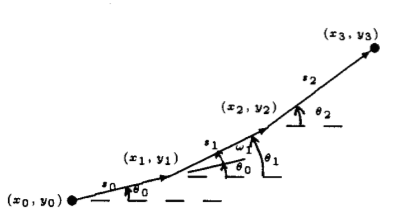
\includegraphics[scale=0.8]{fig1} 
\caption{Dead-Reckoning} 
\end{figure}

\begin{center}
$\theta_k = \sum_{i=0}^k \omega_i$
\end{center}

\section{Sensori}

I sensori disponibili in uno smartphone sono diversi e variano da modello a modello, alcuni sono implementati in maniera hardware (MEMS), altri generano dati mediante algoritmi, quindi in maniera software. 

Nella piattaforma Android possiamo suddividerli in quattro macroaree \cite{K9}:
\begin{itemize}
\item Motion Sensors: include tutti i sensori che misurano le forze di accelerazione e le forze rotazionali come accelerometro, giroscopio, sensore di gravità. Tutte le forze vengono misurate relativamente ai 3 assi.
\item Environmental Sensors: include tutti i sensori che misurano i parametri ambientali come temperatura, pressione atmosferica, illuminazione, umidità. Quindi: termometro, barometro, igrometro e sensore di luminosità.
\item Position Sensors: questi sensori determinano la posizione del device nello spazio come il sensore di orientamento, di prossimità e il magnetometro.
\item Location Sensors: sono indispensabili per la geolocalizzazione del device ed hanno un'accuratezza variabile a seconda della tecnologia, delle condizioni atmosferiche e dalla presenza di ostacoli. Abbiamo: GPS e A-GPS(5m - 10m) \cite{K10}; WIFI e Network Position (10m - 35km).
\end{itemize}

\begin{figure}[h] 
\centering 
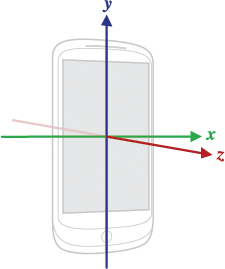
\includegraphics[scale=0.8]{fig2} 
\caption{Sistema delle coordinate} 
\end{figure}

\subsection{MEMS}
MEMS (Micro Electro-Mechanical Systems) è la tecnologia grazie alla quale è possibile realizzare sensori integrati nello smartphone.\\
Un dispositivo MEMS ha un fattore di miniaturizzazione molto elevato e le dimensioni sono contenute, nell'ordine di pochi millimetri cubi di volume.\\
Questo sistema integra dispositivi meccanici, elettrici ed elettronici.\\
La parte meccanica comprende i sensori veri e propri, piccoli chip in grado di misurare fenomeni di natura meccanica, magnetica ed ambientale.\\
Gli elementi meccanici ed elettronici sono integrati in uno substrato di silicio. La parte elettronica del sistema elabora i dati e comunica con lo smartphone. \cite{K14}

\subsection{Accelerometro}
In uno smartphone abbiamo tre accelerometri, ognuno dei quali misura l'accelerazione del device lungo uno dei tre assi. L'unità di misura è $m/s^2$.

\begin{figure}[h!]
\centering 
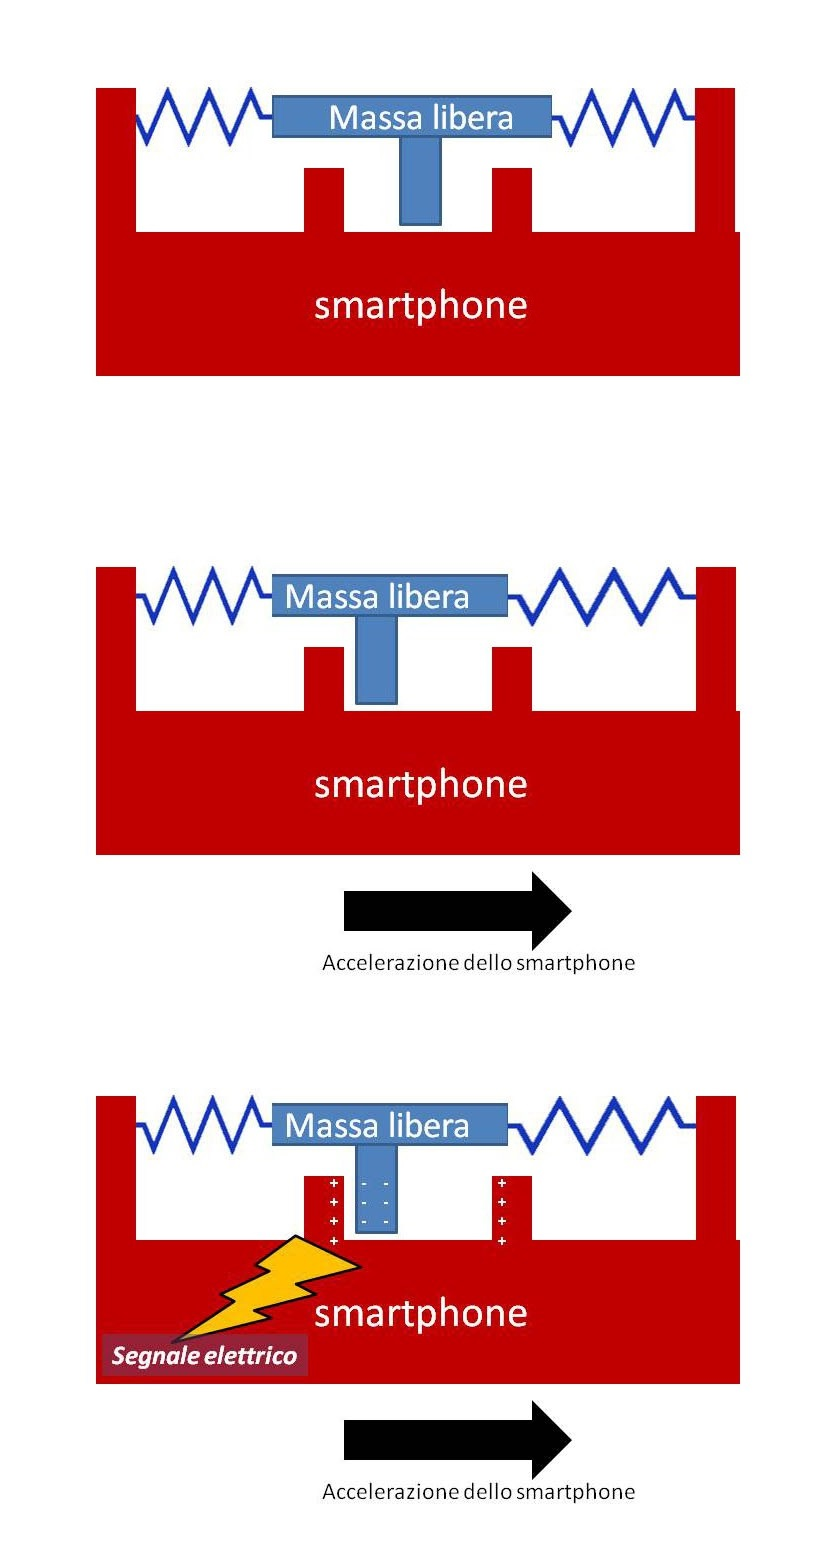
\includegraphics[scale=0.2]{fig4} 
\caption{Accelerometro MEMS} 
\end{figure}
In figura 1.3 possiamo vedere lo schema di funzionamento di un accelerometro MEMS. Abbiamo una massa libera al centro del sensore, collegata alle estremità da una molla per parte ad una parte esterna e fissa alla struttura del device. Quando c'è un'accelerazione, la massa rimane ferma mentre la parte esterna si muove contraendo le molle e facendo in modo che la massa vada a contatto con le armature dell'accelerometro generando un segnale elettrico. 

Nei valori misurati dall'accelerometro è inclusa la forza di gravità, infatti ponendo lo smartphone su un tavolo vediamo che l'accelerometro relativo all'asse Z rileva un'accelerazione pari a 9,8 $m/s^2$.
Per avere valori corretti bisogna capire anche come è orientato nello spazio il device, tramite il giroscopio e applicare un filtro passa-alto per rimuovere la forza di gravità dai tre assi e isolare quindi l'accelerazione lineare.

Mediante l'accelerometro e il calcolo della sua magnitudo possiamo determinare accelerazioni e decelerazioni, quindi capire quando e in che modo un'autovettura frena o accelera e di conseguenza capire anche quando è presente un cambio di velocità del mezzo. \cite{K1, K2, K3, K4, K5, K6}

\begin{center}
$ magnitude = \sqrt{ x^2 + y^2 + z^2}$
\end{center}

\subsection{Giroscopio}
Il giroscopio è un dispositivo che misura la velocità angolare del device intorno ai suoi 3 assi. L'unità di misura è $rad/s$. 

Il funzionamento del giroscopio si basa su ciò che afferma la legge di conservazione del momento angolare, la quale afferma che il momento angolare L di un sistema è costante nel tempo se è nullo il momento delle forze esterne che agiscono su di esso.

Per momento angolare si intende il prodotto vettoriale tra il vettore che congiunge un punto del device con un punto dell'asse intorno al quale il device ruota ed il vettore corrispondente alla quantità di moto, ossia $m \cdot v$.
\begin{center}
$\overrightarrow{L} =  \overrightarrow{r} \times \overrightarrow{p}$
\end{center}

\begin{figure}[h!]
\centering 
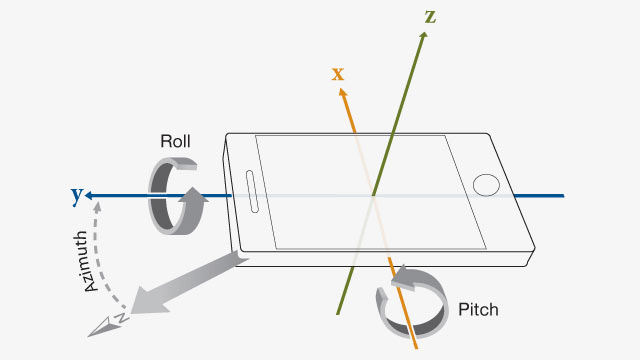
\includegraphics[scale=0.6]{fig6} 
\caption{Giroscopio} 
\end{figure}

Come vediamo nella figura 2.4, l'orientamento del device si può esprimere mediante la velocità rotazionale intorno ai suoi 3 assi, nello specifico, la velocità angolare intorno all'asse x è denominata Pitch, intorno all'asse y è denominata Roll, intorno all'asse z è denominata Yaw mentre l'orientamento del device rispetto al nord magnetico è denominato Azimuth.


Con il giroscopio possiamo determinare l'orientamento del device nello spazio, questa informazione è fondamentale per interpretare correttamente i valori prodotti da altri sensori, come l'accelerometro.
E' un tipo di sensore che non molti smartphone posseggono, è possibile però, simulare il sensore mediante i valori ottenuti dal magnetometro e dall'accelerometro mediante il calcolo delle matrici rotazionali, questo concetto verrà spiegato nel capitolo riguardante l'implementazione del progetto Android.
\subsection{Magnetometro}
Il magnetometro è un dispositivo che misura l'intensità del campo magnetico relativamente ai suoi 3 assi. L'unità di misura è $\mu T$. 


Mediante il magnetometro possiamo determinare la magnitudo del campo magnetico e la direzione del device rispetto al nord magnetico.

\begin{center}
$ magnitude = \sqrt{ x^2 + y^2 + z^2}$
\end{center}
Dove per x, y e z intendo i valori rilevati lungo i rispettivi assi.


\begin{center}
$directionRad = atan2(x,y)$
\end{center}


In questa maniera ottengo la direzione in radianti del device, successivamente trasformo il valore in maniera che il nord magnetico sia a $ \pi / 2$ invece che a 0. Nel caso che la direzione in radianti sia minore di 0, allora sommo ad essa  $2\pi $. \\
Infine trasformo il valore da radianti a gradi:

\begin{center}
$directionGrad = directionRad * 180/ \pi$
\end{center}

La magnitudo in un ambiente privo di fonti magnetiche non potrà mai raggiungere lo zero ma si avvicinerà a valori di circa 30-40 $\mu T$, questo è dovuto al campo geomagnetico del pianeta.

\section{GPS}
Il GPS (Global Positioning System) è un sistema di posizionamento satellitare civile gestito dal governo degli Stati Uniti d'America (GSU). Esso permette di ottenere le coordinate geografiche, quindi la geolocalizzazione, di un oggetto.
Ha un livello di accuratezza molto elevato, in ambito militare ha una precisione di circa 1m, in ambito civile di circa 5-10m.

Il sistema è formato da tre segmenti: il segmento spaziale, il segmento di controllo ed il segmento utente. \cite{K15}


Nel segmento spaziale ci sono da 24 a 31 satelliti Navstar che si muovono lungo 6 piani orbitali con una inclinazione di circa 55 gradi rispetto l'equatore, quindi ogni piano orbitale ha almeno 4 satelliti. Da ogni punto della terra sono sempre visibili almeno 4 satelliti, questo in condizioni favorevoli, ossia senza disturbi come edifici o montagne. Ogni satellite dispone di almeno un orologio atomico e trasmette i dati su due frequenze L1(1575,42 Mhz) e L2(1227,60Mhz).


Il segmento di controllo è formato da stazioni di controllo situate in punti diversi del pianeta che si occupano di controllare il funzionamento dei satelliti e degli orologi atomici, la sincronizzazione degli orologi atomici e si occupano della distorsione artificiale (SA, Selective Availability) del segnale per usi civili.


Nel segmento utente fanno parte tutti i dispositivi che fungono da ricevitori GPS.
\begin{figure}[h!]
\centering 
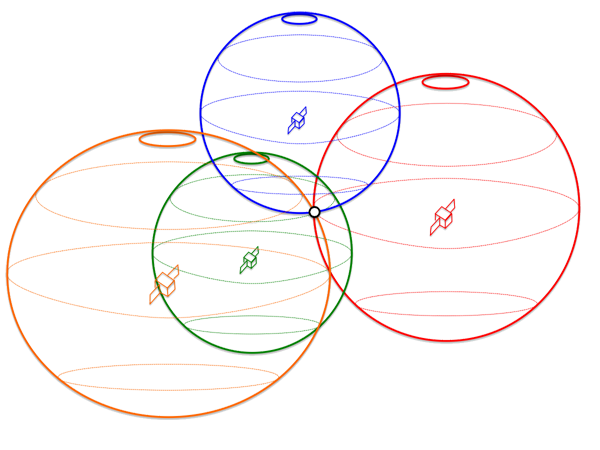
\includegraphics[scale=0.6]{fig8} 
\caption{Punto GPS calcolato mediante 4 satelliti. \cite{K16}} 
\end{figure}


Il sistema si basa sulla tecnica della trilaterazione. 


Le coordinate geografiche sono calcolate a partire dal tempo $ \Delta T $ che ci mette il segnale radio a compiere il tragitto satellite-device. Moltiplicando $ \Delta T $ per la velocità della luce otteniamo la distanza. 

Per conoscere la posizione abbiamo bisogno della distanza di almeno 4 satelliti.

\section{Wi-Fi}
Il Wi-Fi è una tecnologia che permette ai dispositivi di trasmettere dati in maniera wireless, quindi senza l'ausilio di cavi. Si basa sulle specifiche dello standard IEEE 802.11.1

Oltre a permettere di accedere ad una rete locale è possibile connettersi tramite un access point ad Internet e trasmettere dati a dei server remoti.

Una rete Wi-Fi può essere identificata tramite il suo SSID (Service Set IDentifier). Il SSID consiste in 32 byte che contengono il nome della rete in formato human-readable. Nel caso un device si connettesse ad una determinata rete, l'SSID può essere utile nel geolocalizzarlo. 
Ad esempio, se un device invia dei dati mediante la rete Wi-Fi Almawifi possiamo dedurre che il device sia nei pressi di una struttura universitaria.\\
Il BSSID, invece, è un identificatore univoco, consiste nel MAC address dell'access point. \\
Il RSSI invece indica l'intensità del segnale, dalla quale possiamo dedurre e stimare la distanza del device dall'access point. L'unità di misura è dBm.

La quasi totalità delle reti private ha dei meccanismi di sicurezza che servono a prevenire accessi da parte di device non autorizzati. 
Abbiamo per esempio WPA (Wireless Protected Access) e WEP (Wired Equivalent Privacy).

\begin{figure}[h!]
\centering 
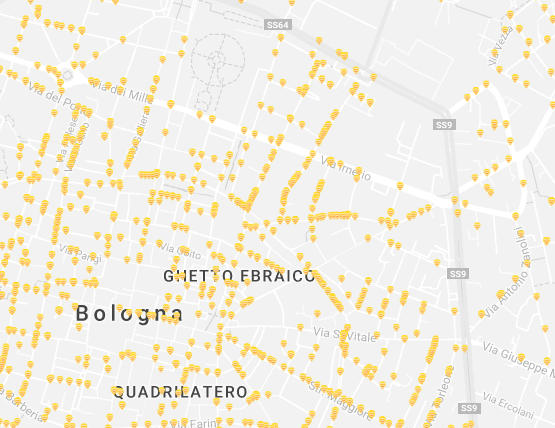
\includegraphics[scale=0.6]{fig7} 
\caption{Hotspot Free a Bologna, dati forniti da fon.com \cite{K16}} 
\end{figure}

Al giorno d'oggi è sempre più facile trovare delle Open-Network \cite{K11}, ossia reti liberi alle quali ci si può collegare gratuitamente. Molti comuni, istituzioni, aree commerciali offrono reti a cui collegarsi liberamente.



\section{OpenStreetMap}
OpenStreetMap (OSM) \cite{K12} è un progetto collaborativo open-data che offre un servizio cartografico.\\
OpenStreetMap è stato fondato nel 2004 da Steve Coast e ad ora è usato da molti servizi come Flickr, Strava, WolframAlpha e tanti altri \cite{K13}.

Essendo un progetto open-data è possibile scaricare in locale od usufruire delle API per effettuare query e sviluppare i propri progetti. I dati sono in formato OSM XML.

Gli elementi fondamentali che compongono il \textit{conceptual data model of the physical world} di OpenStreetMap sono:
\begin{itemize}
\item Node: Un nodo consiste in un punto nello spazio, ed è definito da un nodeId univoco, latitudine e longitudine. I nodi possono essere usati per identificare la forma di un edificio o per comporre strade.\\
I nodi possono avere ulteriori tag, come per esempio "highway", "entrance", "natural", etc.\\
I tag sono formati da un insieme di coppie chiave-valore. \\

\begin{figure}[h] 
\centering 
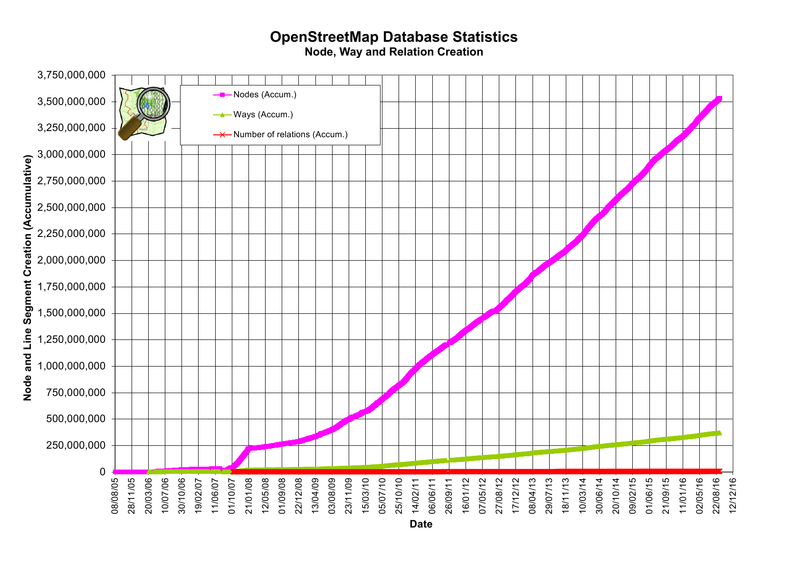
\includegraphics[scale=1]{fig3} 
\caption{Statistiche OpenStreetMap - 2016} 
\end{figure}
\item Way: una way è una lista ordinata di nodi. E' composta da 2 a 2000 nodi. Una way può essere di diversi tipi: chiusa quando l'ultimo nodo è collegato al primo; può essere aperta nel caso di strade; può essere un'area quando delimita una porzione di terreno, se è un area è anche chiusa.\\
Ogni way ha un wayId univoco, una lista di nodi e diversi tag. I più ricorrenti sono "highway", "name", "area", "oneway" e "maxspeed".
\item Relation: una relation è formata da uno o più tags e da un insieme di nodi/way o altre relation che vengono usate per definire relazioni logiche o geografiche tra più elementi. Può essere usata, per esempio, per definire le fermate di un autobus o le stazioni ferroviarie di una determinata linea.
\end{itemize}
\newpage
\section{Grafi}
Un paese, una provincia o addirittura tutto il pianeta può essere inteso come un enorme grafo pesato.

Un nodo del grafo può rappresentare un'intersezione, ossia un punto geografico in cui convergono più strade. Mentre un arco del grafo può rappresentare la strada che collega due intersezioni.
 
Il peso che diamo ad ogni arco può essere o la distanza tra le due intersezioni o il tempo che ci si mette mediamente ad attraversarlo interamente, dipende dai contesti di utilizzo.

In questo modo è facile implementare diversi algoritmi di visita partendo da un nodo di partenza.

Implementando un grafo tramite liste di adiacenza, una DFS (depth-first search) ha una complessità computazionale pari a $\Omega(|V| + |E|) $ dove per $\left|V \right|$ si intende il numero di nodi del grafo e con $\left| E \right|$ il numero di archi.

%%%%%%%%%%%%%%%%%%%%%%%%%%%%%%%%%%%%%%%%%non numera l'ultima pagina sinistra
\clearpage{\pagestyle{empty}\cleardoublepage}
\chapter{Progettazione ed implementazione}                %crea il capitolo
%%%%%%%%%%%%%%%%%%%%%%%%%%%%%%%%%%%%%%%%%imposta l'intestazione di pagina
\lhead[\fancyplain{}{\bfseries\thepage}]{\fancyplain{}{\bfseries\rightmark}}
Il progetto di tesi è composto da due parti distinte:

\begin{itemize}
\item Un'applicazione Android in grado di rilevare uno spostamento del mezzo, di registrare dati dai sensori inerziali e di inviare quest'ultimi al server tramite una connessione Wi-Fi.
\item Un server sviluppato in Python in grado di ricevere dati dall'applicazione Android, interpretarli usando le API di OpenStreetMap e calcolare la posizione del mezzo mediante diversi algoritmi.
\end{itemize}

\begin{figure}[h]
\centering 
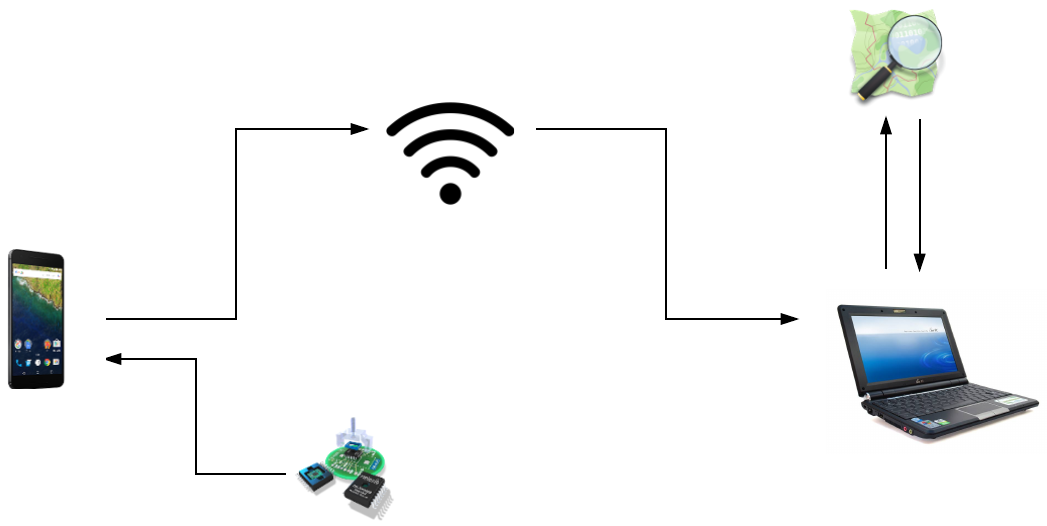
\includegraphics[scale=0.4]{fig10} 
\caption{Schema di funzionamento del progetto.} 
\end{figure}
\newpage
\section{Applicazione Android}
L'applicazione è stata scritta in Java, mediante Android Studio. \\
La versione minima di SDK supportata è la 19 (KitKat) garantendo il corretto funzionamento dell'applicazione su circa l'86,7 \% dei device in uso \cite{K17}.

\begin{figure}[h!]
\centering 
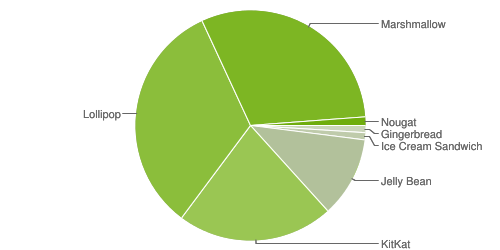
\includegraphics[scale=0.6]{fig11} 
\caption{Statistiche relative alle versioni di Android installate nei device. Dato aggiornato al 6 Febbraio 2017.} 
\end{figure}

\subsection{Concept}
L'idea di base del progetto è quella di implementare un localizzatore inerziale che funga da antifurto per mezzi di trasporto. L'applicazione deve essere installata su un device Android, il quale deve essere posizionato in maniera salda e stabile al mezzo.

Si presuppone che il device sia posizionato in maniera tale che l'Azimuth del device sia uguale all'Azimuth del mezzo di trasporto. In un possibile sviluppo futuro si potrebbe calcolare l'orientamento al momento dell'inizializzazione e considerare questo offset nel momento in cui si analizzano i dati.


L'applicazione una volta avviata si mette in attesa che il mezzo venga rubato, per riconoscere il furto e quindi lo spostamento del mezzo, comincia a rilevare ed analizzare i dati provenienti dall'accelerometro.

La fase di inizializzazione consiste nell'ottenere un unico dato, ossia le coordinate geografiche del mezzo parcheggiato. Siccome il mezzo sul quale è posizionato il dispositivo è fermo, la velocità è pari a 0 km/h e siccome presupponiamo che l'Azimuth del device sia pari all'Azimuth del mezzo non è nemmeno importante capire come è orientato il device all'interno del veicolo.


Dopo che l'applicazione ha rilevato il furto, comincia a registrare i dati generati dai sensori e prova a collegarsi ad una rete Wi-Fi, in caso di avvenuta connessione invia i dati ad un server remoto.
\newpage
\subsection{Implementazione}
L'applicazione è composta da due Activity, ognuna delle quali corrisponde ad una diversa modalità di utilizzo dell'applicazione. Una volta lanciata l'applicazione l'utente potrà cambiare la modalità di utilizzo mediante un pulsante posto in alto a destra sulla AppBar.
\begin{itemize}
\item \textbf{Anti-Theft Mode}\\
E' la modalità di utilizzo in cui l'applicazione funge da antifurto. 

L'utente dovrà posizionare il device e premere il pulsante "Activate" che attiverà il motion detection. Questa modalità implementa il funzionamento descritto nel paragrafo riguardante al concept dell'applicazione.

\item \textbf{Test Mode}\\
Questa modalità mi è servita per costruirmi un dataset utile allo sviluppo della parte server. In questa modalità l'utente dovrà posizionare il device
nel punto desiderato e quando vuole far partire la registrazione dovrà premere sul pulsante "Start", mentre dovrà premere il pulsante "Stop" per interrompere la registrazione e salvare il file contenente i dati generati dai sensori in locale sul device. Inoltre l'utente clickando sulle label corrispondenti alle coordinate potrà visualizzare il punto corrispondente su Google Maps, potrà vedere il nome del file appena esportato ed il contenuto di quest'ultimo.
\end{itemize}

\begin{figure}[h!]
\centering 
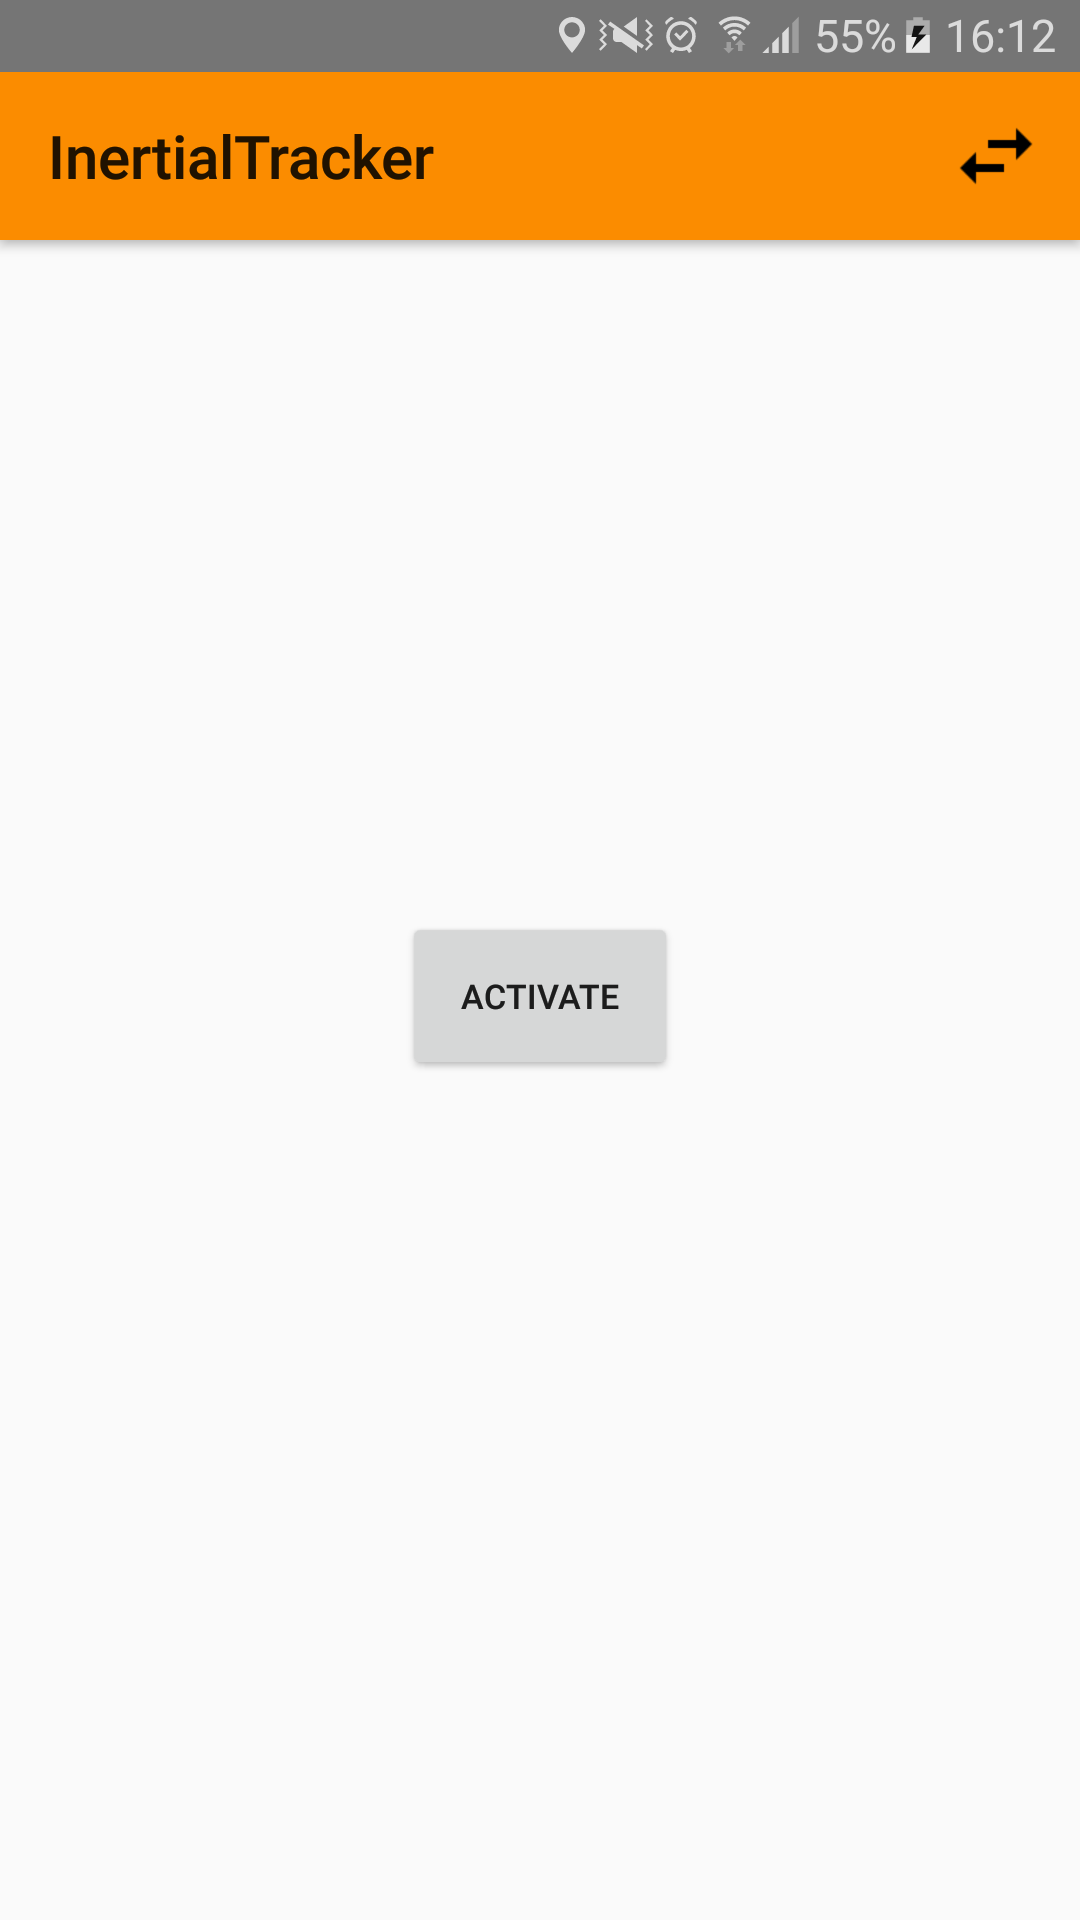
\includegraphics[scale=0.1]{TestActivity} 
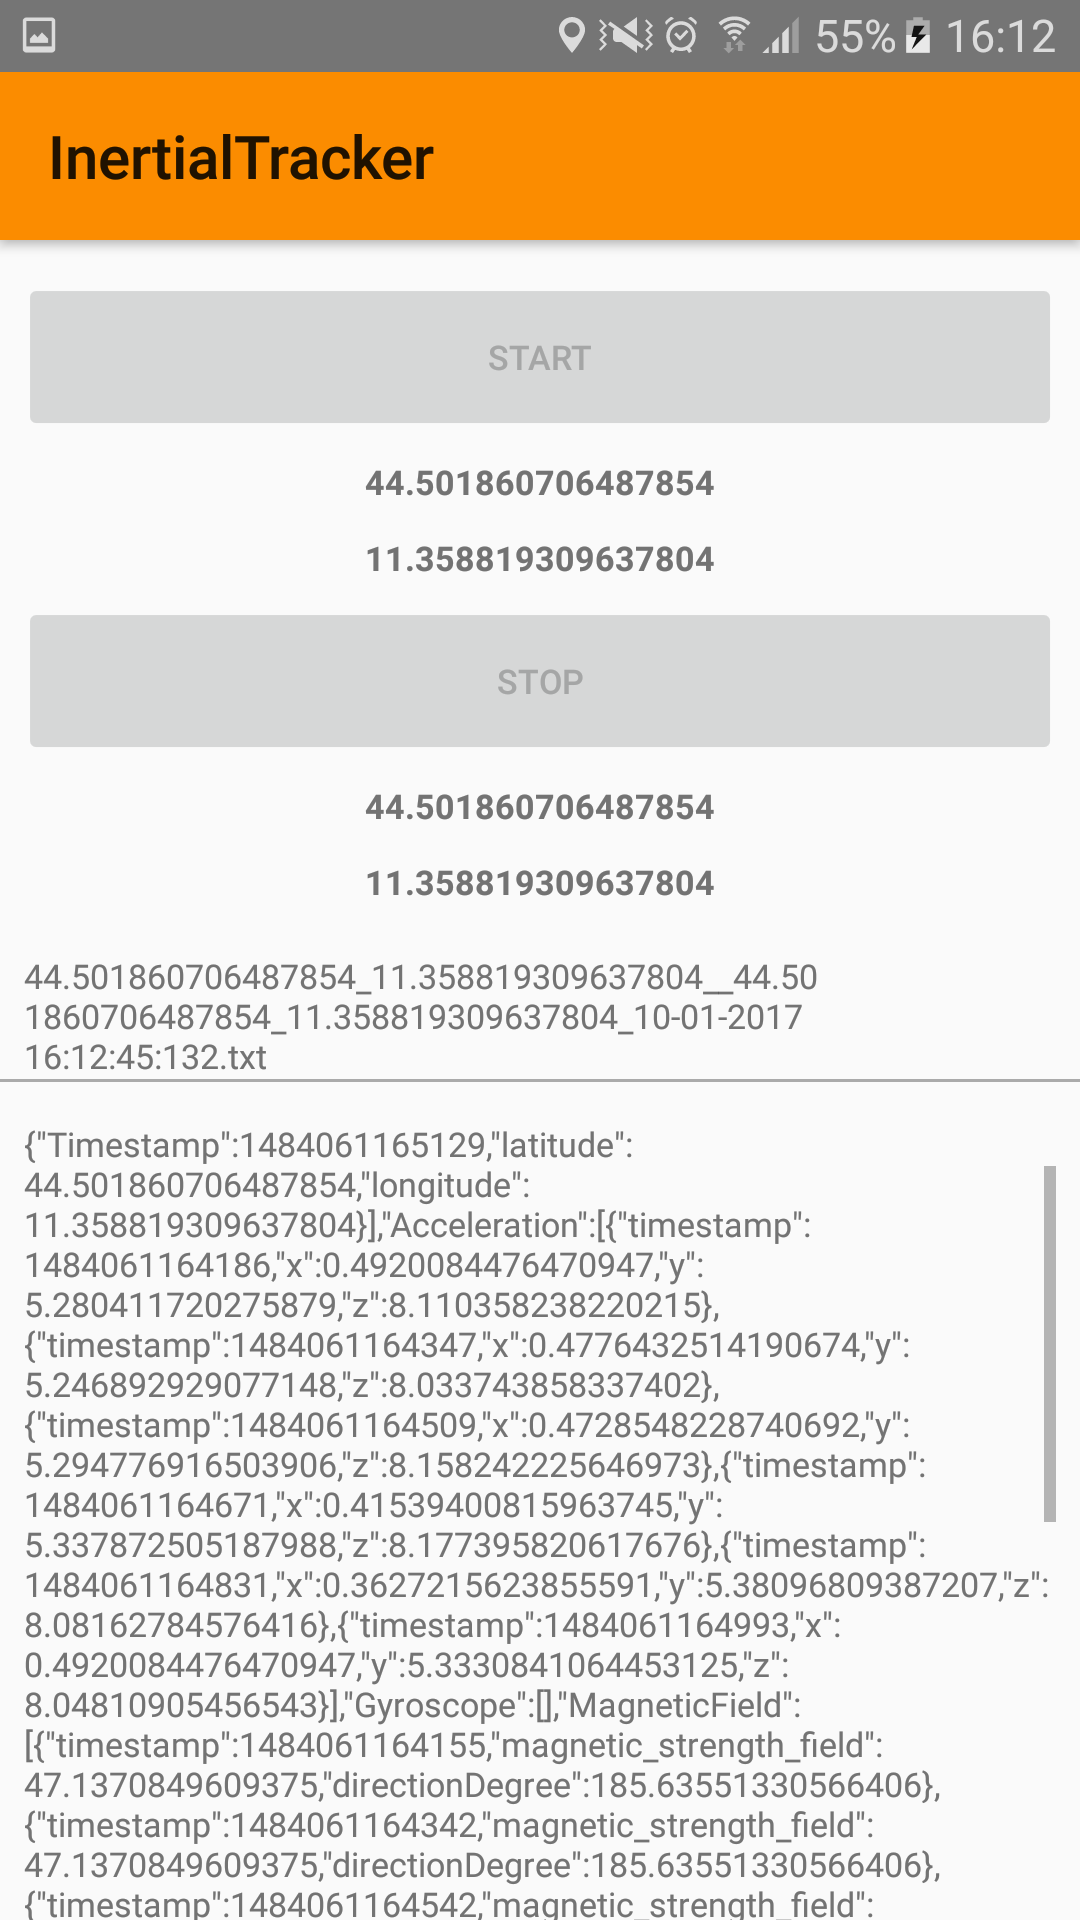
\includegraphics[scale=0.1]{MainActivity} 
\caption{Anti-Theft Mode a sinistra, Test Mode a destra.} 
\end{figure}

L'applicazione presenta diverse classi, ora andremo a presentarle nel dettaglio.
\subsubsection*{MotionDetection}
La classe MotionDetection si occupa di rilevare un movimento del mezzo. Viene invocata solamente nella Anti-Theft Mode quando l'utente preme su "Activate". \\
MotionDetection implementa l'interfaccia SensorEventListener e chiede al SystemService tramite il SensorManager la possibilità di leggere i dati generati dall'accelerometro ad una frequenza pari a 5Hz.
Ogni volta che l'applicazione rileva una minima accelerazione ne calcola la magnitudo dalla quale sottrae la forza di gravità

\begin{center}
$ magnitude = \sqrt{ x^2 + y^2 + z^2} - gravity$
\end{center}

Se la magnitudo è maggiore rispetto ad una certa costante, l'applicazione capisce che il mezzo su cui è posizionato il device ha subito un cambiamento di velocità e quindi è stato spostato dal punto originario. Dopo diverse prove ho impostato la sensibilità del MotionDetection ad un valore pari ad 1 in maniera che l'applicazione sia in grado di minimizzare sia i falsi positivi che i falsi negativi, quindi, che riesca ad interpretare come un furto lo spostamento del mezzo ma che non riesca ad interpretare come tale, ad esempio, le vibrazioni prodotte dal passaggio di mezzi pesanti nelle immediate vicinanze.

Nel momento in cui l'applicazione rileva lo spostamento del mezzo, vengono lanciati in esecuzione i due Service, il primo relativo alla registrazione dei dati provenienti dai sensori, il secondo relativo all'invio dei dati al server.	

\subsubsection*{gpsPosition}
gpsPosition è la classe adibita alla geolocalizzazione del device. Mediante il LocationManager ottiene dal SystemService la possibilità di ottenere informazioni dal Location\_Service. \\
Ogni volta che viene invocata registra la posizione corrente del device nel jsonObject.

\subsubsection*{jsonUtils}
Questa classe gestisce il jsonObject contenente tutti i valori ottenuti dai sensori. Nel caso in cui l'applicazione sia in esecuzione in modalità Test Mode, il jsonObject viene salvato in un file .json nella memoria locale del device. Nel caso in cui l'applicazione sia in esecuzione in modalità Anti-Theft Mode, invece, il jsonObject viene passato al Service adibito all'invio dei dati al server.

\subsubsection*{parallelIntentService}
ParallelIntentService \cite{K18} estende la classe Service ed implementa un comportamento simile agli IntentService.
E' stata utile per gestire due Service parallelamente in due thread differenti e non entrambi nell'UI thread.

\subsubsection*{httpRequest}
Per gestire le richieste HTTP ho usato Android Asynchronous Http Client \cite{K19}, una comoda libreria per gestire richieste HTTP sia in maniera asincrona che sincrona.
La richiesta HTTP avviene nello stesso thread in cui avviene la chiamata ad essa e fino a che la richiesta non è conclusa, il thread relativo si mette in wait, facendo quindi una comunicazione di tipo sincrono.

\subsubsection*{logData}
logData è un Service ed estende la classe parallelIntentService, ed implementa SensorEventListener.\\
Lo scopo della classe è quello di registrare tutti i dati provenienti dai sensori e salvarli mediante i metodi forniti da jsonUtils in un unico jsonObject.

Tramite il SensorManager l'applicazione ottiene dal SystemService l'accesso al SENSOR\_SERVICE. Il SensorManager comincia ad elaborare i dati provenienti da diversi sensori: accelerometro, magnetometro e giroscopio.

Oltre a questi sensori, l'applicazione calcola la matrice rotazionale del device tramite i valori raccolti dal magnetometro e dall'accelerometro. Una volta ottenuta la matrice rotazionale tramite il getRotationMatrix, otteniamo un'array di valori i quali indicano l'orientamento del device tramite getOrientation.
I valori ottenuti saranno: Azimuth, Pith e Roll.
Il calcolo dell'orientamento tramite la matrice rotazionale è indispensabile per i dispositivi che non dispongono del giroscopio e per ottenere un valore di Azimuth corretto esente da errori relativi all'orientamento del dispositivo.

L'analisi dei dati generati dal sensore avviene ad una frequenza di 20Hz.


\subsubsection*{checkSend}
checkSend è un Service ed anche esso estende la classe parallelIntentService.
checkSend si occupa dell'invio dei dati al server. Ogni volta che il thread relativo è in esecuzione la classe controlla se il Wi-Fi è abilitato ed attivo. In caso di risposta affermativa, controlla se il dispositivo è attualmente connesso ad una rete Wi-Fi mediante il metodo checkConnection().

checkConnection() mediante il ConnectivityManager ottiene le informazioni relative alla network attiva, se è presente una network attiva ed è di tipo Wi-Fi, controlla se il device è connesso, nel caso lo fosse scrive sul jsonObject le informazioni relative alla network e invia i dati al server.
Se il dispositivo non è collegato ad alcuna rete Wi-Fi, tramite il metodo searchFreeWifi() ottengo una lista delle rete Wi-Fi disponibili, le filtro escludendo le reti che hanno politiche di accesso e restituisco la network con il maggior valore di RSSI, ossia quella in cui il segnale è maggiore. 
Nel caso searchFreeWifi() restituisca una network, l'applicazione proverà a collegarsi, in caso di avvenuta connessione, salverà nel jsonObject le informazioni relative alla network e invierà i dati al server.

L'invio dei dati è gestito dal metodo sendData(), il quale farà una richiesta HTTP di tipo POST al server mediante la classe httpRequest.

\newpage
\section{Server}
Il server è stato sviluppato in Python 3.

Come l'applicazione Android, anche esso ha una duplice modalità di utilizzo. Abbiamo la modalità che si interfaccia con l'applicazione Android in Anti-Theft Mode, quindi riceve i dati, li analizza e genera dei possibili punti geografici in cui il mezzo si potrebbe trovare tramite i vari algoritmi. L'altra modalità di utilizzo è quella che si interfaccia con la Test Mode dell'applicazione Android, ossia cerca di valutare l'efficienza dei vari algoritmi confrontando le posizioni calcolate dagli algoritmi con la posizione reale di fine registrazione. 
Il funzionamento è il medesimo.

I valori con cui gli algoritmi lavorano sono esclusivamente i valori relativi all'Azimuth.

\subsection{Generazione del grafo}

Il server, appena riceve i dati, ottiene le informazioni relative al punto geografico di partenza, quindi latitudine, longitudine e timestamp relativo all'inizio della registrazione.
Una volta ottenute le coordinate geografiche di partenza avviene il reverseGeocoding, esso consiste in una query a OpenStreetMap dalla quale otteniamo l'ID del nodo più vicino alle coordinate geografiche date in input. La query viene eseguita mediante Python Overpass Wrapper (Overpy). Dalla query otteniamo una lista di Nodi all'interno di un certo raggio, da questa lista filtriamo i nodi che appartengono ad una strada, controllando se da ogni nodo è possibile raggiungerne almeno una, successivamente cerchiamo il più vicino alle coordinate di partenza.
Una volta ottenuto l'ID del nodo, il sistema si calcolo una BoundingBox, ossia un'area rettangolare dove l'ID del nodo trovato in precedenza si trova esattamente all'intersezione delle due diagonali. 

In seguito, il sistema si interfaccia direttamente con le API di OpenStreetMap e scarica il file OSM-XML relativo alla BoundingBox. La richiesta avviene mediante urllib. Una volta ottenuto l'XML, esso viene salvato per poterlo usare in futuro in maniera più rapida per eventuali nuove localizzazioni. L'XML viene parsato mediante BeautifulSoup.


La fase successiva consiste nella generazione del grafo pesato mediante NetworkX, il quale è una libreria Python che fornisce un'implementazione di un grafo mediante una struttura dati di tipo dictionary basata su liste di adiacenza.

Il file OSM-XML è un file contenente tutte le informazioni riguardanti ad una determinata area geografica. Per interpretare tali informazioni ho implementato due classi: Intersection e Road.

La classe Intersection è la classe relativa alle intersezioni stradali, ossia i nodi in cui convergono più strade. Ogni oggetto di tipo Intersection ha un ID, una latitudine ed una longitudine.


La classe Road è la classe relativa alle strade, ossia i segmenti che collegano tra loro due intersezioni. Ogni oggetto di tipo Road ha un ID, il nome della strada, il tipo di strada ed il limite di velocità. 


Ho implementato diverse funzioni indispensabili per costruire e navigare il grafo. Abbiamo \textit{getListIntersection} che prende in input un oggetto di tipo Road e restituisce una lista di Intersection presenti nella strada. \textit{getListWayReached} che prende in input un oggetto di tipo Intersection e restituisce la lista di Road che convergono in esso. \textit{getCommonWay} è una funzione che ha come parametri due oggetti di tipo Intersection e restituisce, se esiste, l'oggetto Road che li congiunge.


La funzione adibita alla costruzione del grafo è una funziona ricorsiva che ha come parametri il grafo stesso, l'ID del nodo che si sta analizzando, le coordinate del nodo Root, il raggio, ossia la distanza in metri massima tra il nodo Root e il nodo da aggiungere, e l'oggetto parsato mediante BeautifulSoup corrispondente al file OSM-XML.

Per ogni nodo che analizziamo ricaviamo mediante il costruttore di Intersection le coordinate geografiche, ne calcoliamo la distanza dal nodo Root e nel caso la distanza sia minore rispetto al raggio della BoundingBox continuiamo ad analizzarlo.

Otteniamo una lista di strade, le quali si possono raggiungere direttamente dal nodo, nel caso il nodo facesse parte della shape della strada allora la lista avrà un solo elemento, ossia la strada stessa, nel caso in cui il nodo sia un intersezione allora avremmo tutte le strade che intersecano l'incrocio.

Successivamente, per ognuna di queste strade, otteniamo la lista di intersezioni e se l'intersezione non fa già parte del grafo allora otteniamo il nodo relativo all'intersezione, la distanza tra le due intersezioni e le informazioni sulla strada che le collega. In seguito, aggiungiamo nel grafo l'arco tra il nodo corrente e il nodo trovato, dando come peso la distanza in metri tra i due nodi, successivamente viene richiamata la funzione ricorsiva dando come nodo da analizzare il nodo appena trovato.

Una volta generato il grafo lo esportiamo per poterlo usare in future computazioni successive in maniera più rapida.

La fase seguente è quella relativa agli algoritmi di visita del grafo e viene descritta in maniera più accurata nel prossimo paragrafo.
\newpage
\subsection{Algoritmi di visita}
I dati ottenuti dall'applicazione Android servono per generare indicazioni che gli algoritmi di visita del grafo useranno per prendere decisioni su che arco percorrere.
Le indicazioni vengono generate tramite una funzione \textit{getAzimuth} che prenderà come parametri i dati stessi, la lunghezza della finestra temporale e il numero di quadranti in cui dividere la circonferenza. La funzione scorrerà i dati ottenuti ed aggregherà i valori contenuti nella medesima finestra temporale, ne calcolerà la media, il quadrante in cui l'Azimuth medio ricade e la durata dell'indicazione che sarà pari alla lunghezza della finestra temporale, ad eccezione dell'ultima indicazione.
La lista delle indicazioni è implementata come uno stack.

Ora passiamo a descrivere gli algoritmi:

\subsubsection{Backtrack}
Questo algoritmo corrisponde ad una visità in profondità del grafo (DFS). E' una funzione ricorsiva che ha come parametri il grafo da visitare, l'ID del nodo corrente, la lista delle indicazioni ed il numero di quadranti. Ad ogni istanza si controlla se esistono indicazioni da consumare e se il grafo contiene il nodo da analizzare, in caso di risposta affermativa settiamo il nodo come visitato, otteniamo l'indicazione da consumare e la lista dei nodi adiacenti al nodo corrente. Per ogni nodo adiacente, se non è stato già visitato, ne ricaviamo le coordinate e calcoliamo il bearing tra il nodo corrente e il nodo in questione. Se il nodo è nello stesso quadrante dell'indicazione da consumare allora ottengo la distanza tra i due nodi, il limite di velocità della strada che li collega e calcolo i secondi da consumare, presupponendo che il mezzo vada ad una velocità pari al limite di velocità della strada. 

Se i secondi consumati sono minori rispetto ai secondi rimanenti nell'indicazione da seguire, mi calcolo la differenza e riaggiungo l'indicazione alla lista delle indicazioni. Se invece i secondi da consumare sono maggiori rispetto alla finestra temporale, ottengo una nuova indicazione e se il quadrante di quest'ultima è uguale al quadrante della precedente allora consumo i secondi rimanenti da questa nuova indicazione.

La computazione si blocca quando la visita arriva ad un nodo che non ha più nodi da visitare o quando le indicazioni sono già state consumate tutte. Ogni volta che la computazione si blocca, l'ultimo nodo visitato viene aggiunto ad una lista che corrisponde ai possibili output.

\subsubsection{BestDecision}
BestDecision è un algoritmo iterativo. La visita parte dal nodo Root e la gestione delle indicazioni è uguale all'algoritmo Backtrack. La visita avviene usando un algoritmo decisionale, ad ogni iterazione l'algoritmo valuta tutti i nodi adiacenti al nodo corrente e  per ogni nodo ne calcola il bearing. Viene scelto il nodo il cui bearing si avvicina di più al valore dell'Azimuth dell'indicazione da consumare. 

\subsubsection{RandomDecision}
E' un algoritmo molto simile al BestDecision solo che ogni volta che l'algoritmo deve scegliere il nodo successivo da visitare, filtra i nodi adiacenti escludendo i nodi che si trovano in quadranti diversi da quello indicato dall'indicazione e se i nodi rimanenti sono più di uno, allora effettua una scelta casuale.

\subsubsection{DeadReckoning}
L'algoritmo di DeadReckoning non è un algoritmo di visita del grafo in quanto non si interfaccia con OpenStreetMap e con il grafo che l'algoritmo genera.
E' un algoritmo iterativo e come parametri ha le coordinate di partenza da cui iniziare a computare, la lista delle indicazioni e il limite di velocità con cui fare i calcoli.
L'algoritmo itera fino a che ha indicazioni da consumare, per ogni indicazione calcola i metri corrispondenti allo spostamento, il bearing di esso e successivamente calcola le nuove coordinate.


%%%%%%%%%%%%%%%%%%%%%%%%%%%%%%%%%%%%%%%%%non numera l'ultima pagina sinistra
\clearpage{\pagestyle{empty}\cleardoublepage}
\chapter{Performance Evaluation}                %crea il capitolo
%%%%%%%%%%%%%%%%%%%%%%%%%%%%%%%%%%%%%%%%%imposta l'intestazione di pagina
\lhead[\fancyplain{}{\bfseries\thepage}]{\fancyplain{}{\bfseries\rightmark}}
\section{Fase Preliminare}
Per effettuare i test ho raccolto alcune tracce mediante l'applicazione Android nella modalità TestMode.

Per ognuna di queste tracce ho eseguito gli algoritmi di visita variando di volta in volta alcuni parametri:
\begin{itemize}
\item Numero di quadranti: 2, 4, 8.
\item Ampiezza della finestra temporale: 20sec, 10sec, 5sec, 1sec.
\item Algoritmo di visita: Backtrack, BestDecision, RandomDecision e DeadReckoning.
\item Limite di velocità: 30, 50, 70, 90.
\end{itemize}
Per un totale di 192 risultati per ogni traccia.

Ho usato il limite di velocità in maniera parametrica e non sfruttando le API di OpenStreetMap in quanto in ambito urbano la media della velocità è più prossima ai 30km/h che ai 50km/h. Questo perchè nel calcolare i metri percorsi ignoro le accelerazioni e le decelerazioni e in ambito urbano sono molto più influenti rispetto all'ambito extra-urbano.

Per cercare di capire le differenze di prestazione degli algoritmi in caso di ambito urbano ed extraurbano, le tracce non comprendono più di un tipo di ambito diverso. 

Ogni volta che un algoritmo calcola un risultato calcola anche l'errore in metri di quest'ultimo, ossia la distanza tra le coordinate calcolate e quelle reali. Successivamente lo salva su un file CSV, generando quindi un unico file contenente tutti i risultati di tutte le tracce.
Per valutare l'efficienza degli algoritmi, oltre all'errore in metri, è stato generato anche l'errore in percentuale in base alla distanza del tracciato effettivamente percorso. Questo dato è stato calcolato ed inserito manualmente.

Dal momento che l'algoritmo di Backtrack genera una lista di possibili output, ho tenuto in considerazione il nodo più vicino alle coordinate reali. In un possibile sviluppo futuro si può pensare a come trovare il migliore output da questa lista.

Per la RandomDecision invece, per ogni combinazione di parametri è stato eseguito l'algoritmo 20 volte e calcolata la media delle distanze di ogni coordinata trovata.

Nel algoritmo di DeadReckoning gli unici parametri significativi sono il limite di velocità e l'ampiezza della finestra temporale.

Dopo aver generato il file CSV contenente le informazioni relative a tutte le computazioni, ho implementato uno script in Python, mediante matPlotLib, in grado di generare diversi grafici per cercare di valutare in maniera più accurata i risultati. Nei grafici generati non ho tenuto conto del parametro "limite di velocità" in quanto non è oggetto della valutazione e ho tenuto conto del miglior risultato ottenuto variando questo parametro.

Le tracce prese in considerazione sono di tipologie differenti, variano per distanza, durata in secondi, numero di curve, contesto urbano o extraurbano.

Nel primo tipo di grafico generato possiamo vedere per ogni traccia l'errore in percentuale di ogni algoritmo. Abbiamo generato 12 grafici, uno per ogni combinazione di numero di quadranti e ampiezza della finestra temporale. I file sull'asse x sono disposti in ordine di maggior distanza percorsa.

Nel secondo tipo di grafico ho calcolato l'errore medio di tutte le tracce in percentuale per ogni singolo algoritmo. Anche in questo caso abbiamo generato 12 grafici. Abbiamo preso in considerazione tutti gli errori rilevati per tipo di algoritmo e non l'errore minimo risultante da una determinata combinazione di limite di velocità, numero di quadranti e ampiezza della finestra temporale.

Nel terzo tipo di grafico abbiamo generato per ogni algoritmo 4 grafici, in ognuno dei quali abbiamo fissato l'ampiezza della finestra temporale, ed analizzato l'andamento dell'errore in metri in relazione alla lunghezza del tracciato effettivamente percorso da ogni traccia, ogni linea del grafico corrisponde ad un numero di quadranti presi in considerazione. In totale abbiamo generato 4 grafici per ogni algoritmo, quindi 16 grafici in totale.

Nel quarto tipo di grafico abbiamo esaminato l'andamento degli errori in metri per ogni algoritmo, fissando il numero di quadranti a 2 e variando l'ampiezza della finestra temporale. Abbiamo generato 4 grafici in totale.

\begin{figure}[H]
\centering 
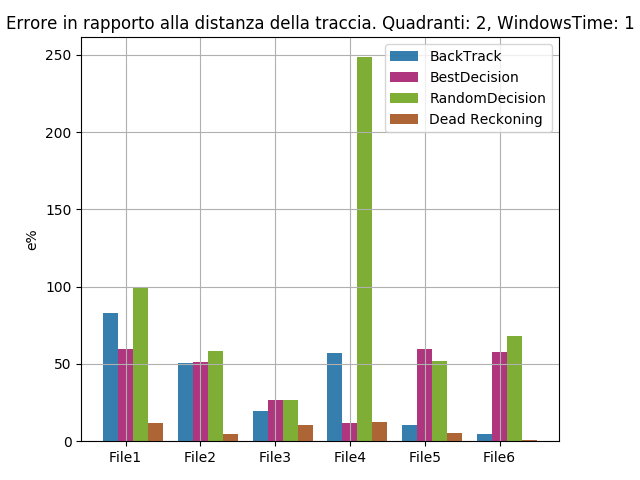
\includegraphics[scale=0.4]{firstChart2-1} 
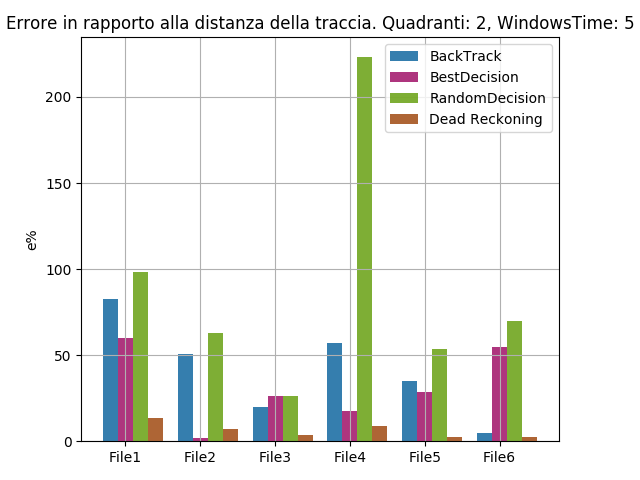
\includegraphics[scale=0.4]{firstChart2-5} 
\end{figure}

\begin{figure}[H]
\centering  
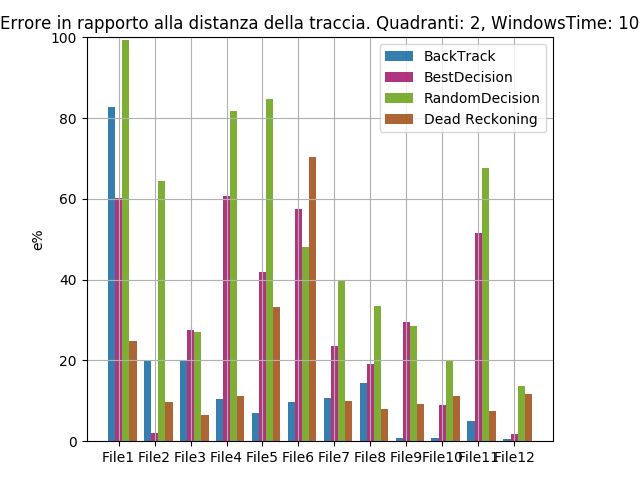
\includegraphics[scale=0.4]{firstChart2-10} 
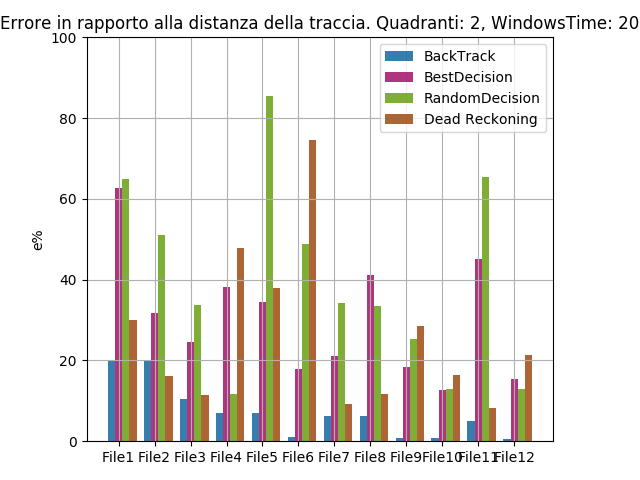
\includegraphics[scale=0.4]{firstChart2-20} 
\end{figure}

\begin{figure}[H]
\centering 
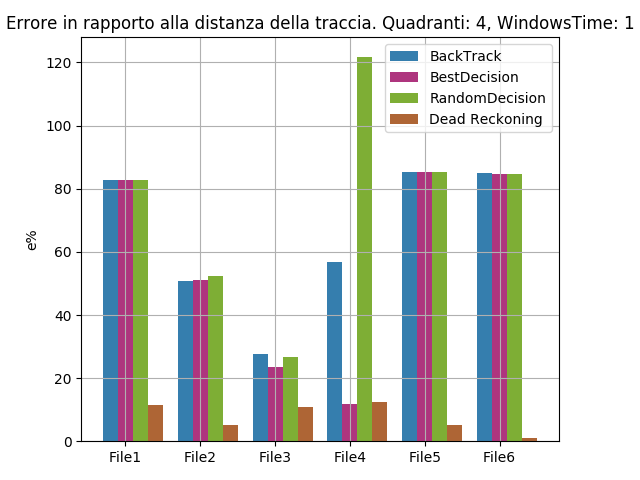
\includegraphics[scale=0.4]{firstChart4-1} 
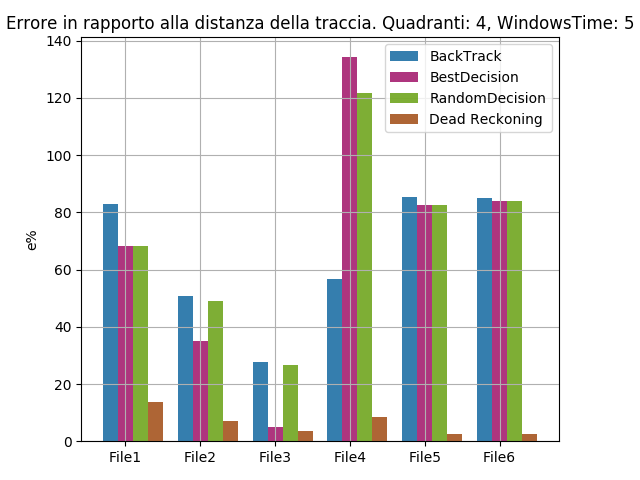
\includegraphics[scale=0.4]{firstChart4-5} 
\end{figure}

\begin{figure}[H]
\centering  
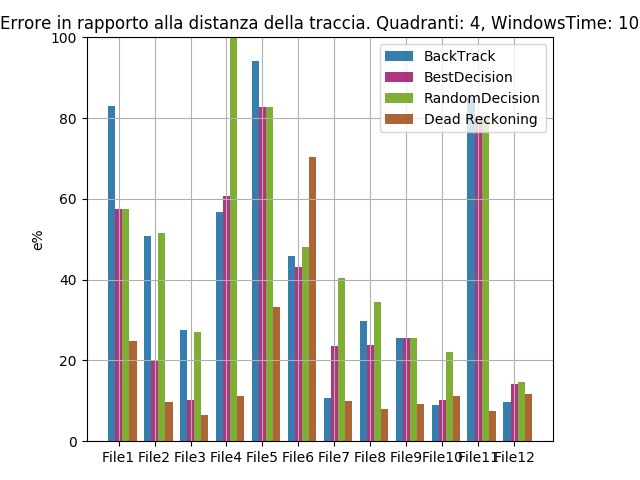
\includegraphics[scale=0.4]{firstChart4-10} 
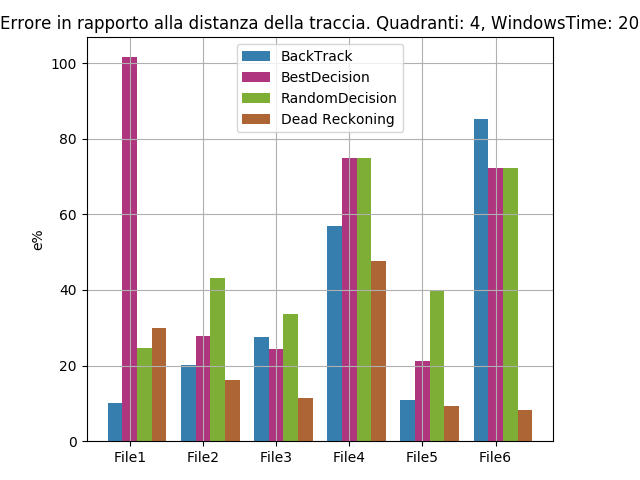
\includegraphics[scale=0.4]{firstChart4-20} 
\end{figure}

\begin{figure}[H]
\centering 
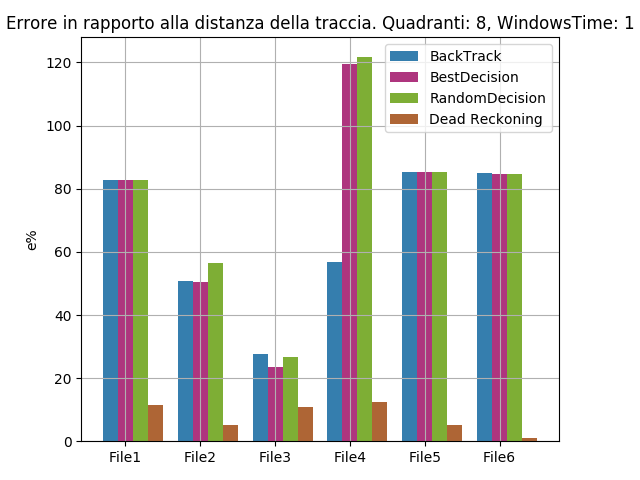
\includegraphics[scale=0.4]{firstChart8-1} 
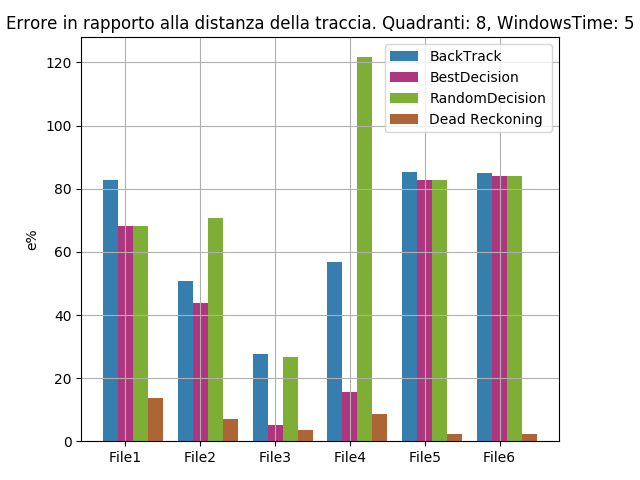
\includegraphics[scale=0.4]{firstChart8-5} 
\end{figure}

\begin{figure}[H]
\centering  
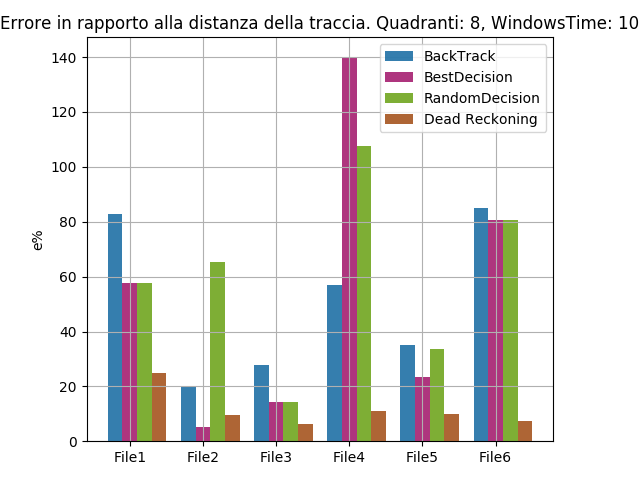
\includegraphics[scale=0.4]{firstChart8-10} 
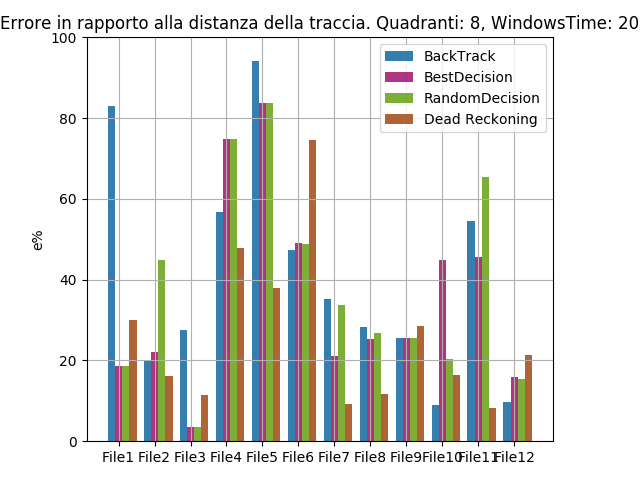
\includegraphics[scale=0.4]{firstChart8-20} 
\end{figure}

\begin{figure}[H]
\centering 
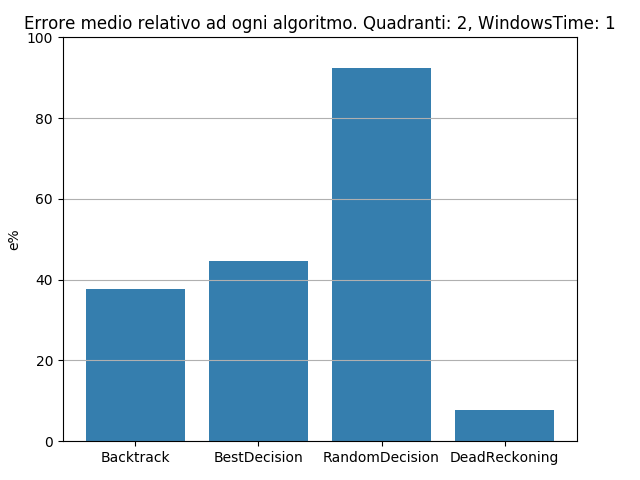
\includegraphics[scale=0.4]{secondChart2-1} 
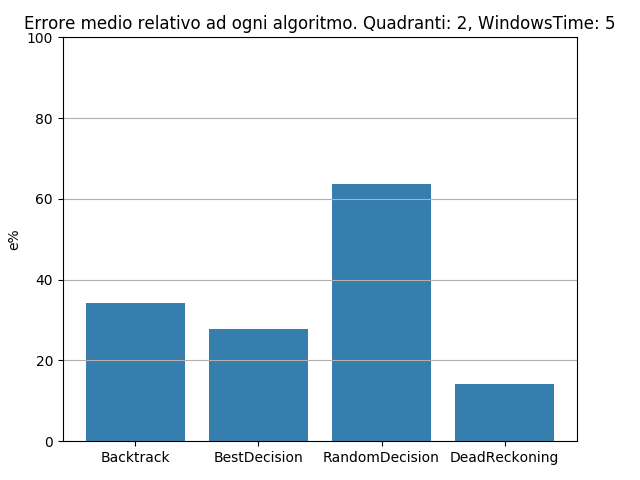
\includegraphics[scale=0.4]{secondChart2-5} 
\end{figure}

\begin{figure}[H]
\centering  
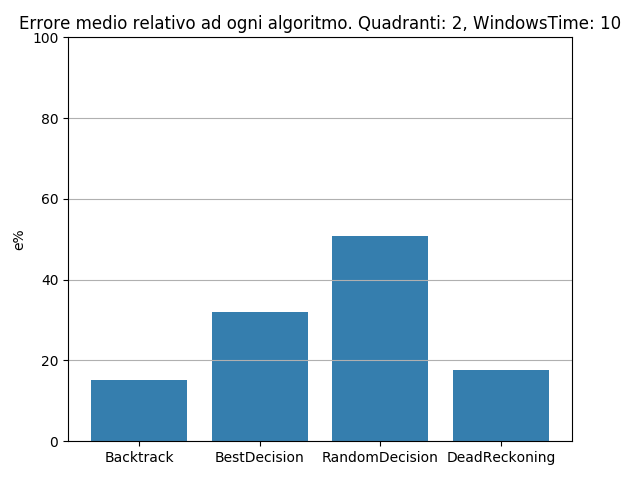
\includegraphics[scale=0.4]{secondChart2-10} 
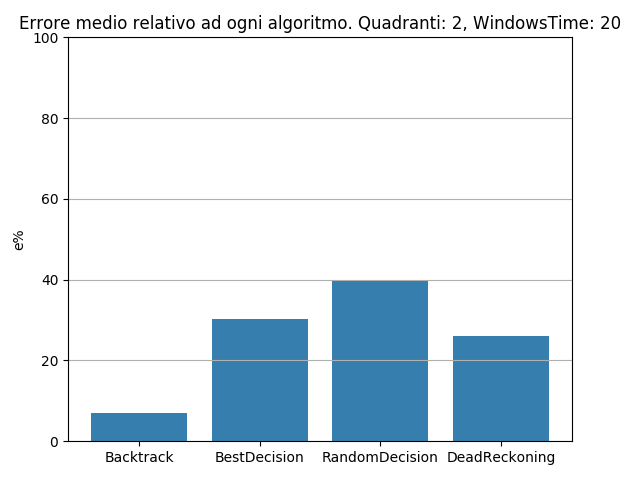
\includegraphics[scale=0.4]{secondChart2-20} 
\end{figure}

\begin{figure}[H]
\centering 
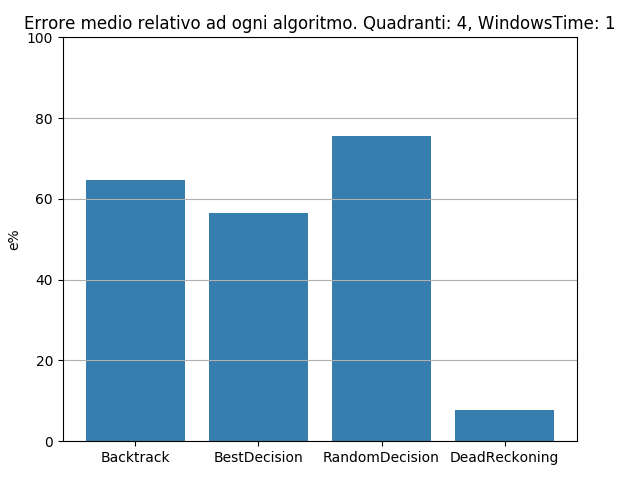
\includegraphics[scale=0.4]{secondChart4-1} 
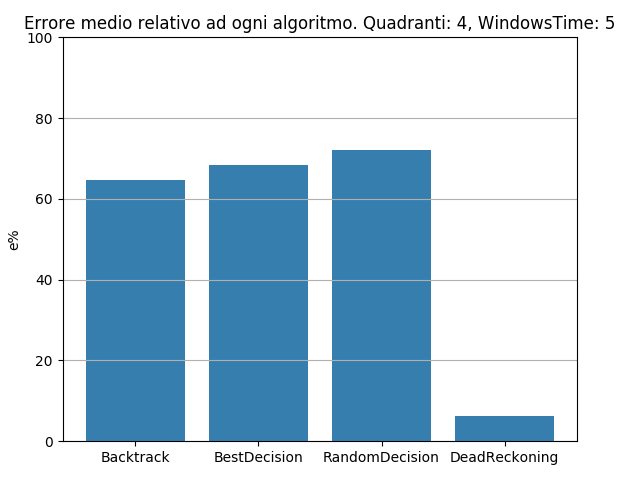
\includegraphics[scale=0.4]{secondChart4-5} 
\end{figure}

\begin{figure}[H]
\centering  
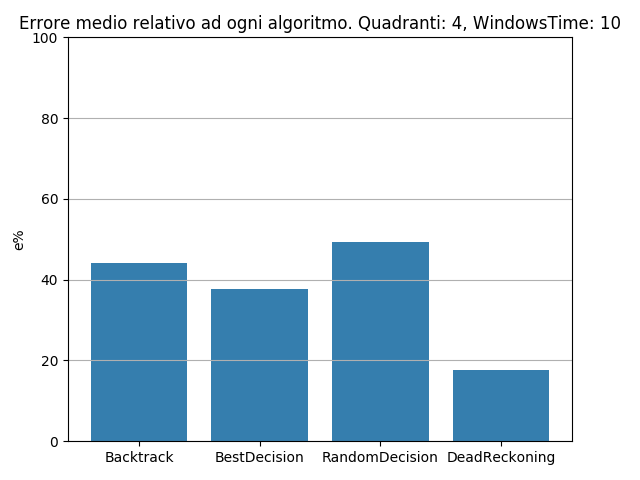
\includegraphics[scale=0.4]{secondChart4-10} 
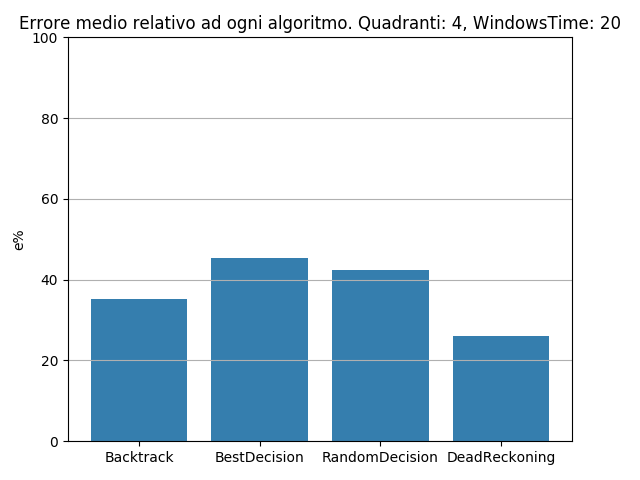
\includegraphics[scale=0.4]{secondChart4-20} 
\end{figure}

\begin{figure}[H]
\centering 
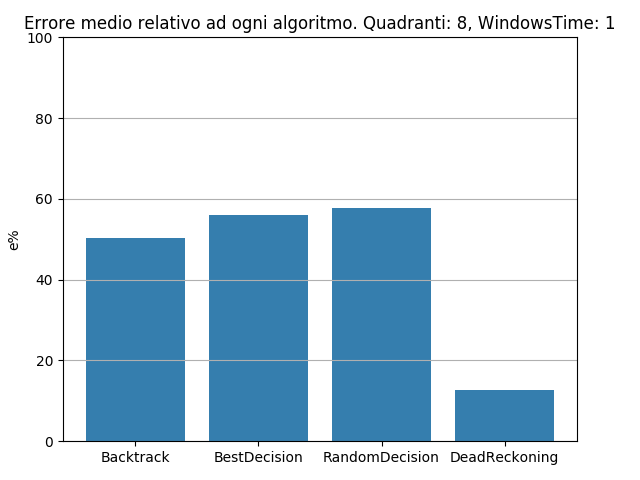
\includegraphics[scale=0.4]{secondChart8-1} 
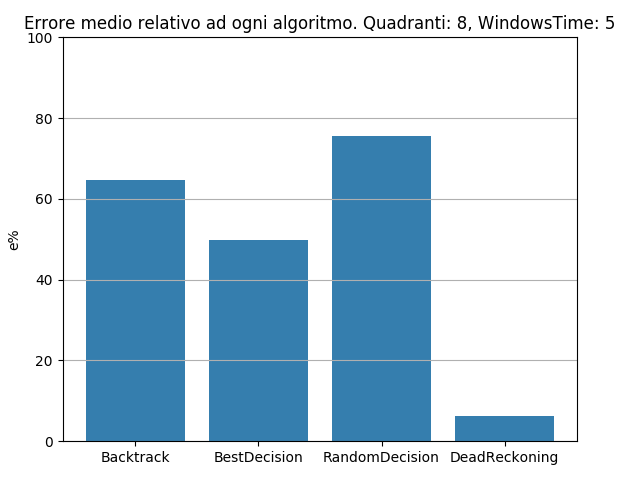
\includegraphics[scale=0.4]{secondChart8-5} 
\end{figure}

\begin{figure}[H]
\centering  
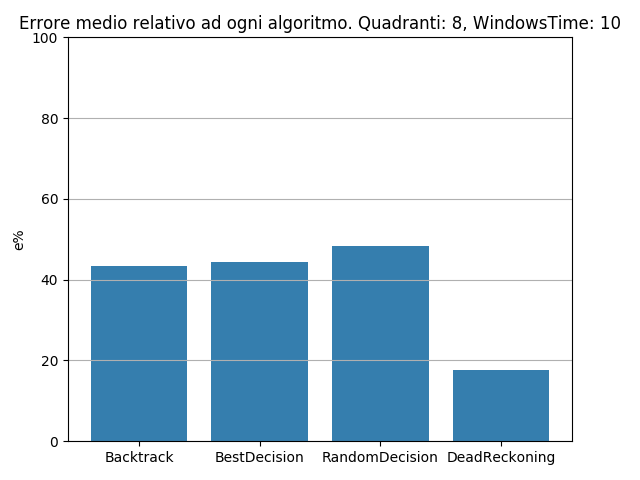
\includegraphics[scale=0.4]{secondChart8-10} 
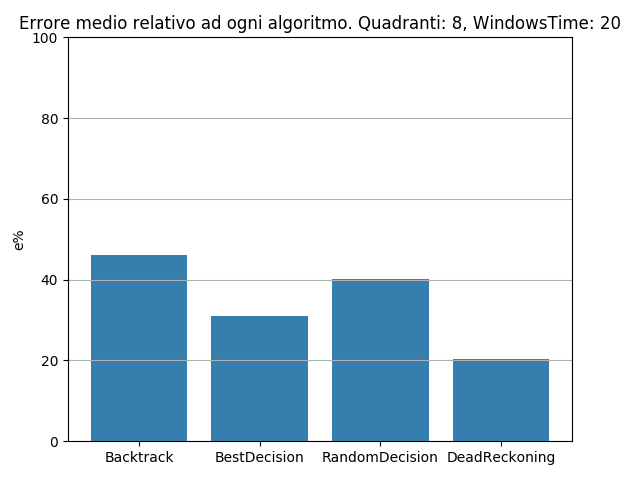
\includegraphics[scale=0.4]{secondChart8-20} 
\end{figure}

\begin{figure}[H]
\centering 
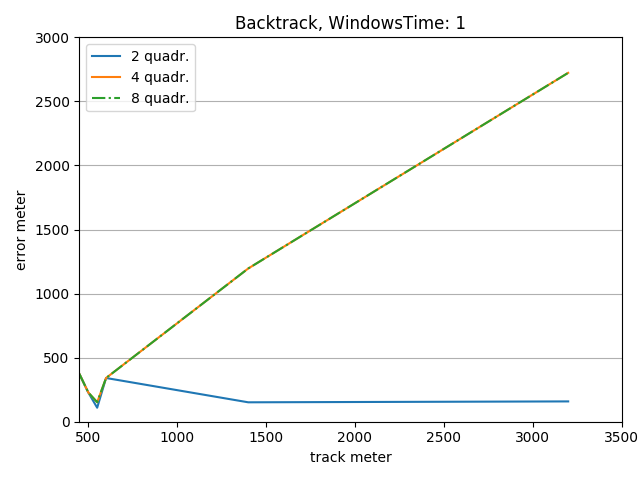
\includegraphics[scale=0.4]{thirdChartBacktrack-1} 
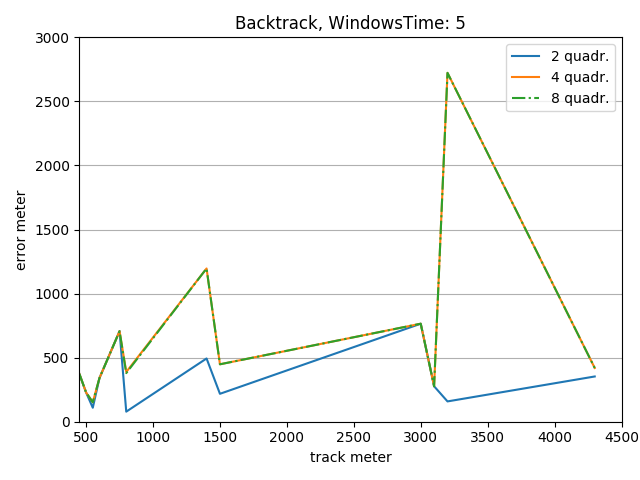
\includegraphics[scale=0.4]{thirdChartBacktrack-5} 
\end{figure}

\begin{figure}[H]
\centering  
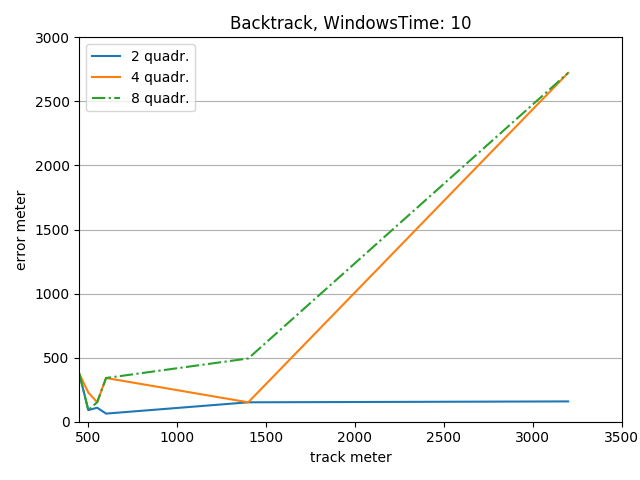
\includegraphics[scale=0.4]{thirdChartBacktrack-10} 
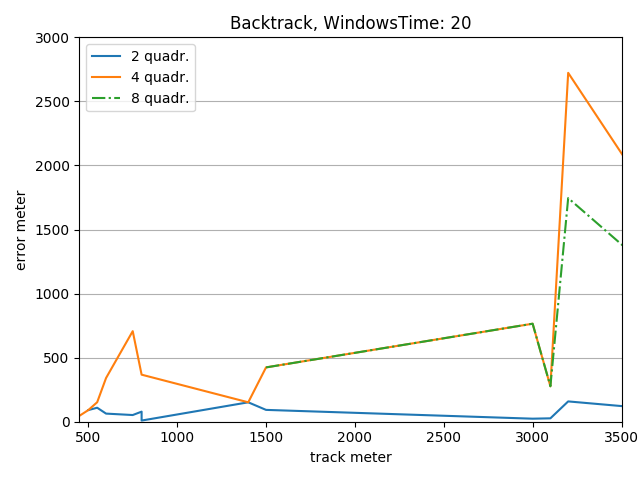
\includegraphics[scale=0.4]{thirdChartBacktrack-20} 
\end{figure}

\begin{figure}[H]
\centering 
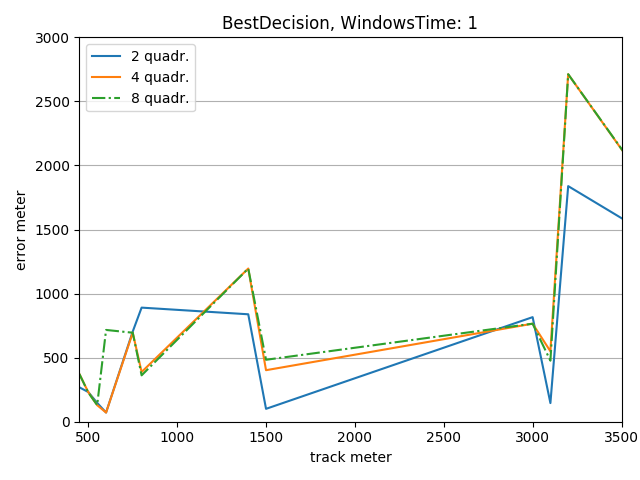
\includegraphics[scale=0.4]{thirdChartBestDecision-1} 
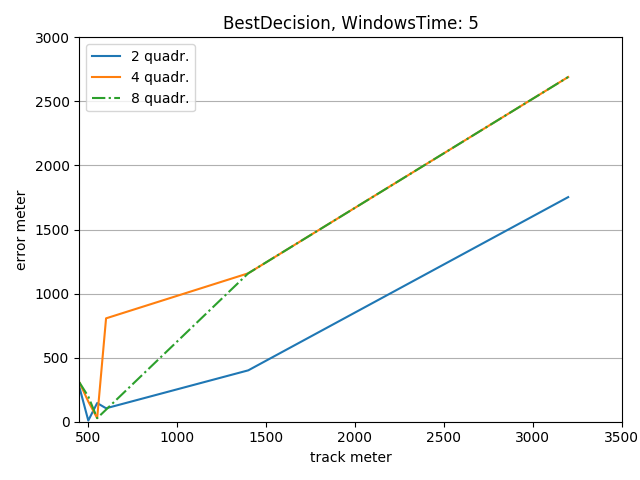
\includegraphics[scale=0.4]{thirdChartBestDecision-5} 
\end{figure}

\begin{figure}[H]
\centering  
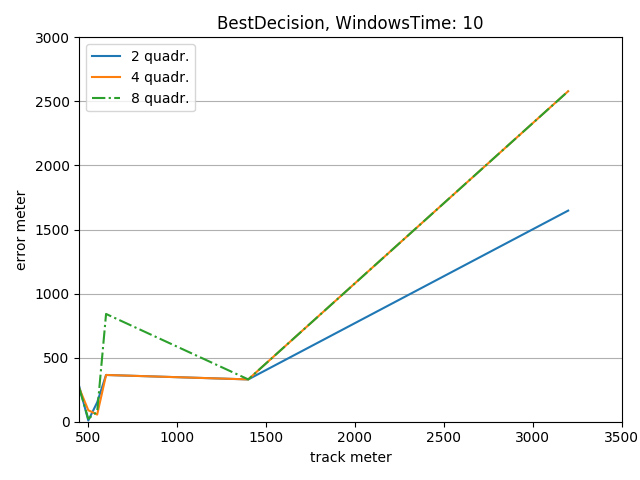
\includegraphics[scale=0.4]{thirdChartBestDecision-10} 
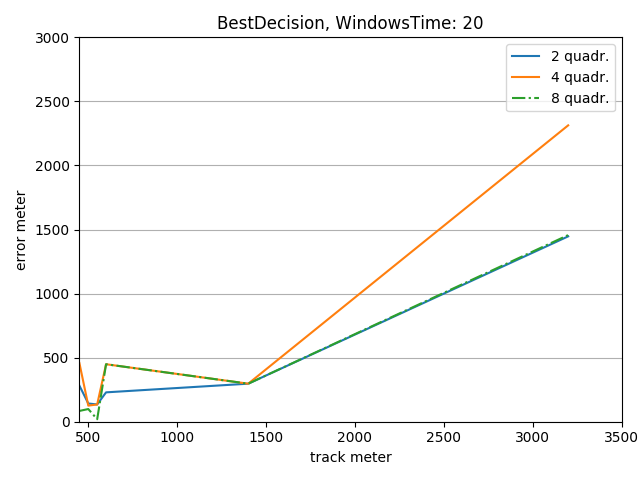
\includegraphics[scale=0.4]{thirdChartBestDecision-20} 
\end{figure}

\begin{figure}[H]
\centering 
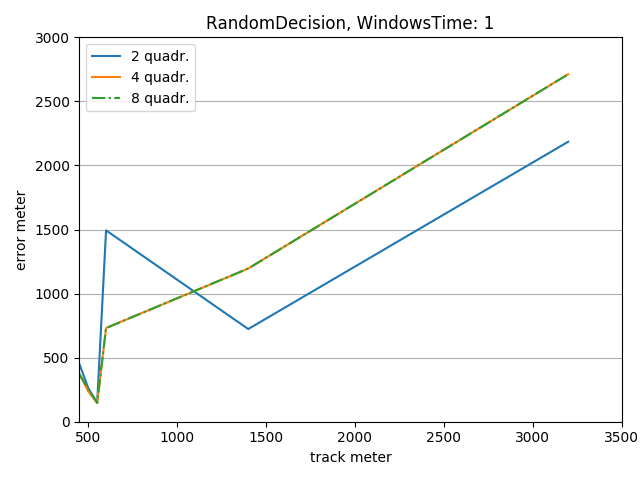
\includegraphics[scale=0.4]{thirdChartRandomDecision-1} 
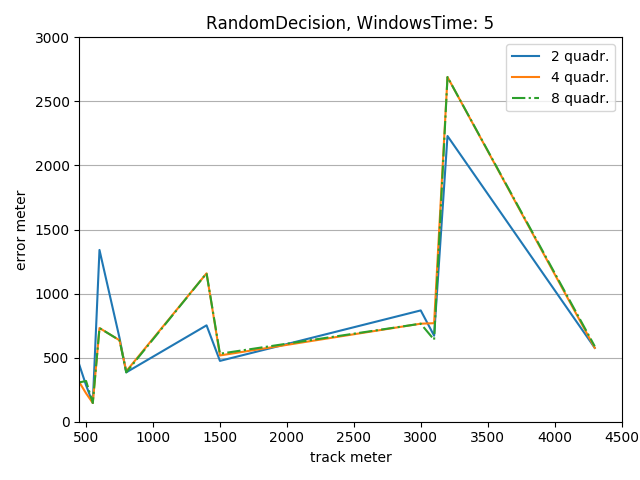
\includegraphics[scale=0.4]{thirdChartRandomDecision-5} 
\end{figure}

\begin{figure}[H]
\centering  
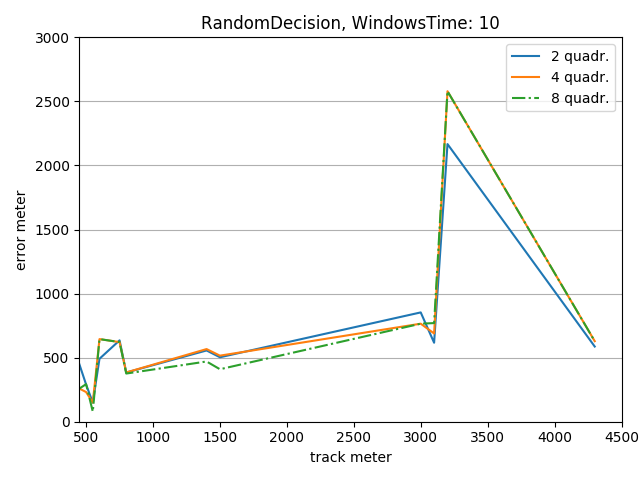
\includegraphics[scale=0.4]{thirdChartRandomDecision-10} 
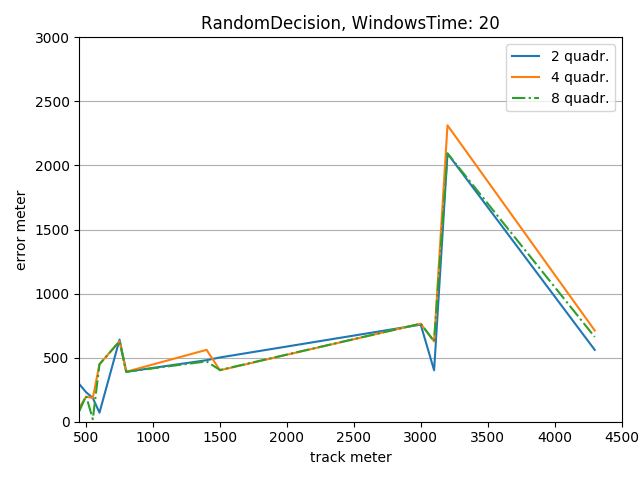
\includegraphics[scale=0.4]{thirdChartRandomDecision-20} 
\end{figure}

\begin{figure}[H]
\centering 
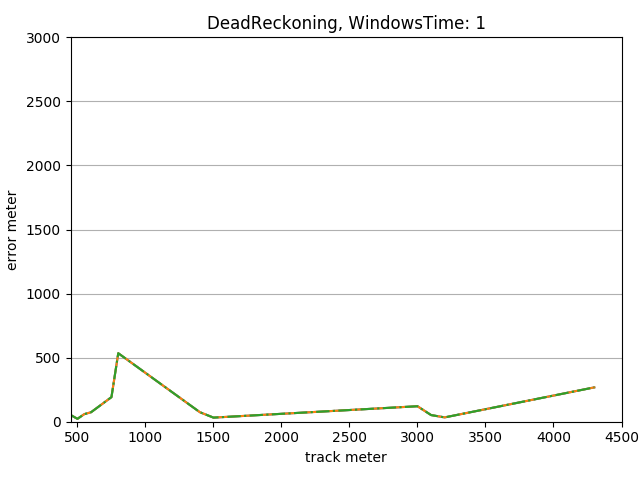
\includegraphics[scale=0.4]{thirdChartDeadReckoning-1} 
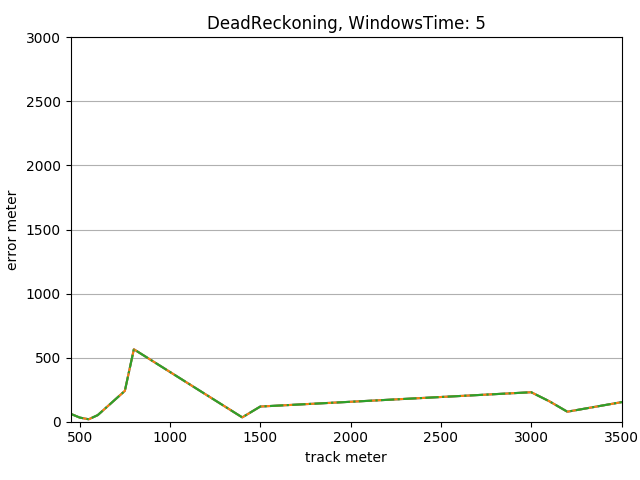
\includegraphics[scale=0.4]{thirdChartDeadReckoning-5} 
\end{figure}

\begin{figure}[H]
\centering  
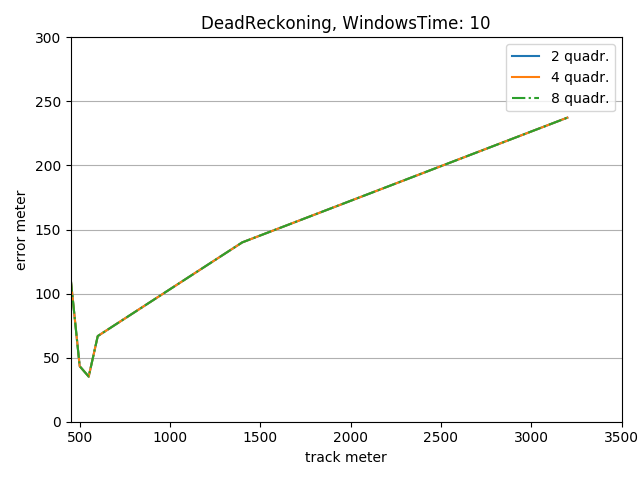
\includegraphics[scale=0.4]{thirdChartDeadReckoning-10} 
\includegraphics[scale=0.4]{thirdChartDeadReckoning-20} 
\end{figure}

\begin{figure}[H]
\centering 
\includegraphics[scale=0.4]{fourChart1} 
\includegraphics[scale=0.4]{fourChart5} 
\end{figure}

\begin{figure}[H]
\centering  
\includegraphics[scale=0.4]{fourChart10} 
\includegraphics[scale=0.4]{fourChart20} 
\end{figure}

\newpage
\section{Analisi dei dati}
In questa sezione analizzeremo le tipologie di grafico generate per poi valutare il comportamento e l'efficienza di ogni algoritmo. Successivamente confronteremo i risultati ottenuti e delineeremo vantaggi e svantaggi di ogni algoritmo a seconda del tipo di traccia e dei parametri impostati ad ogni visita del grafo.

\subsubsection{Grafico 1}
Osservando i grafici relativi agli errori in percentuale rapportati alla distanza reale del percorso effettuato si evince che abbiamo prestazioni differenti a seconda dei numeri di quadranti scelti e a seconda dell'ampiezza della finestra temporale.
Possiamo vedere immediatamente qual è l'algoritmo con le prestazioni peggiori, ossia il RandomDecision che nella quasi totalità delle traccie è l'algoritmo che genera l'errore maggiore, a volte allontanandosi addirittura rispetto al punto di partenza.

\subsubsection{Grafico 2}
La seconda serie di grafici raggruppa tutti i risultati ottenuti da ogni algoritmo con un determinato numero di quadranti e ampiezza della finestra temporale. L'errore medio è stato calcolando facendo la media aritmetica degli errori percentuali e non degli errori in metri.
Da questi grafici possiamo valutare l'efficienza media di ogni singolo algoritmo.

Valutando 2 quadranti possiamo vedere che il comportamento degli algoritmi cambia in modo sostanziale in base al valore della finestra temporale. Con finestre temporali ampie, 20 e 10 secondi, l'algoritmo di Backtracking ha un comportamento medio migliore rispetto al DeadReckoning. In caso di finestre temporali brevi, 1 e 5 secondi, abbiamo che il DeadReckoning si comporta in maniera migliore rispetto all'algoritmo di Backtracking.
Gli algoritmi di BestDecision e RandomDecision hanno in media un comportamento peggiore rispetto agli algoritmi di Backtracking e DeadReckoning. L'algoritmo di BestDecision genera un errore medio del 30\% sia con finestre temporali ampie che con finestre temporali medio-basse. L'algoritmo di RandomDecision ha il suo comportamento migliore con finestre temporali ampie e peggiore con finestre temporali basse.

Aumentando i numeri di quadranti, l'algoritmo di Backtracking continua a comportarsi meglio con finestre temporali ampie rispetto a quelle basse, però l'errore medio aumenta in modo sostanziale favorendo l'utilizzo dell'algoritmo di DeadReckoning. Possiamo vedere anche che aumentando il numero di quadranti le prestazioni del RandomDecision migliorano arrivando a circa lo stesso livello del BestDecision.

\subsubsection{Grafico 3}
Dalla terza tipologia di grafici possiamo vedere come variano gli errori in metri a seconda dei numeri di quadranti utilizzati.

Nell'algoritmo di Backtrack i risultati migliori li possiamo ottenere usando un numero basso di quadranti. Notiamo anche che nel caso migliore, ossia con finestre temporali ampie, l'errore in metri è pressochè costante e si aggira su un valore di circa 200 metri che è un risultato ottimo in caso di percorsi lunghi, peggiore in caso di percorsi inferori ad 1km.

Negli algoritmi di BestDecision e RandomDecision il numero di quadranti scelti è meno rilevante anche se i comportamenti migliori li abbiamo con 2 quadranti.

I grafici relativi all'algoritmo di DeadReckoning non mette in correlazione gli errori rispetto al numero di quadranti ma è utile per analizzare la variazione degli errori in metri in rapporto alla distanza dei percorsi. Con un'ampiezza della finestra temporale pari a 1 secondo possiamo vedere che l'errore in metri è pressochè costante fino a circa 3000 metri per poi cominciare ad aumentare.

\subsubsection{Grafico 4}
Nell'ultima serie di grafici abbiamo analizzato il comportamento dei vari algoritmi confrontandoli fra loro.
Con una finestra temporale breve l'algoritmo migliore è nella quasi totalità dei casi il DeadReckoning, aumentando la lunghezza del percorso la prestazione cala notevolmente.
Con una finestra temporale ampia l'algoritmo migliore è l'algoritmo di Backtracking, esso non peggiora con l'aumentare della distanza del percorso.

\medskip
Ora andremo a riassumere quanto visto e a descrivere il comportamento di ogni algoritmo.

\subsubsection{Backtracking}
L'algoritmo di Backtracking ha il suo comportamento migliore con finestre temporali ampie e con un numero di quadranti ridotto. Mantiene un errore in metri  costante rispetto alla distanza del percorso e quindi l'errore percentuale cala notevolmente in caso di percorsi lunghi. Si comporta in egual maniera sia in contesti urbani che in contesti extraurbani.

\subsubsection{BestDecision}
Questo algoritmo ha anche esso un comportamento migliore con finestre temporali ampie. Non raggiunge mai le prestazioni degli algoritmi di Backtracking e di DeadReckoning. Non è molto affidabile, in quanto basta che sbaglia una svolta in un intersezione o un'uscita in una rotatoria che l'algoritmo continua la visita allontanandosi dal punto di arrivo reale.

\subsubsection{RandomDecision}
Questo algoritmo è una sorta di BestDecision che ogni volta che deve valutare in che arco continuare a computare effettua una scelta casuale tra i possibili archi da poter attraversare. Questo algoritmo è l'algoritmo che ha un comportamento peggiore rispetto a tutti gli altri. Si comporta in maniera migliore con finestre temporali ampie e con un numero di quadranti elevato, questo perchè la scelta casuale avverrà tra un numero minore di archi in cui poter andare e quindi avremo più scelte finali simili tra loro.

\subsubsection{DeadReckoning}
Quest'algoritmo sfrutta esclusivamente i valori ottenuti dai sensori dello smartphone, senza interfacciarsi con OpenStreetMap e con il grafo generato da quest'ultimo. Nonostante la generazione di errori cumulativi ad ogni singola computazione, l'algoritmo si comporta notevolmente meglio con finestre temporali brevi rispetto a quelle ampie, nonostante il numero di computazioni siano ampliamente maggiori.
Con percorsi lunghi oltre 3000m le prestazioni calano a favore del Backtracking che è esente da cali di prestazioni in base alla distanza del percorso. In ambito urbano soffre l'alto numero di cambiamenti di direzione.

\medskip
In conclusione i dati ottenuti dimostrano che l'algoritmo migliore in caso di tragitti medio-brevi, sopratutto in ambito extra-urbano è l'algoritmo di DeadReckoning con una finestra temporale pari a 1 secondo. 

In caso di tragitto medio-lunghi , sopratutto in ambito urbano, l'algoritmo migliore è l'algoritmo di Backtracking con una finestra temporale pari a 20 secondi.

%%%%%%%%%%%%%%%%%%%%%%%%%%%%%%%%%%%%%%%%%non numera l'ultima pagina sinistra
\clearpage{\pagestyle{empty}\cleardoublepage}
%%%%%%%%%%%%%%%%%%%%%%%%%%%%%%%%%%%%%%%%%per fare le conclusioni
\chapter*{Conclusioni}
%%%%%%%%%%%%%%%%%%%%%%%%%%%%%%%%%%%%%%%%%imposta l'intestazione di pagina
\rhead[\fancyplain{}{\bfseries
CONCLUSIONI}]{\fancyplain{}{\bfseries\thepage}}
\lhead[\fancyplain{}{\bfseries\thepage}]{\fancyplain{}{\bfseries
CONCLUSIONI}}
%%%%%%%%%%%%%%%%%%%%%%%%%%%%%%%%%%%%%%%%%aggiunge la voce Conclusioni
                                        %   nell'indice
\addcontentsline{toc}{chapter}{Conclusioni} 

In questo elaborato si è descritto, inizialmente, lo stato dell'arte relativo ai sistemi di navigazione inerziale e a concetti di sensoristica in ambito smartphone, successivamente si è descritto il progetto e lo sviluppo di un applicazione Android, in grado di rilevare un furto e in grado di raccogliere i dati provenienti dai sensori, e un server in grado di computare questi dati ottenuti dall'applicazione ed implementare un sistema di localizzazione mediante quattro algoritmi. La fase successiva è stata quella di generare dei dati per valutare l'efficienza degli algoritmi di localizzazione. Infine si è effettuata un'analisi relativa agli algoritmi al variare di alcuni parametri. Successivamente si è dimostrato quali sono sono gli algoritmi più efficienti in base al percorso, relativamente al contesto e la durata della traccia.

La tesi ha dimostrato che è possibile effettuare una localizzazione di un oggetto mediante, esclusivamente, dati generati da sensori inerziali con un basso margine di errore. 

Negli eventuali sviluppi futuri si potranno incrementare le prestazioni di questi algoritmi disponendo di sensori più precisi e più affidabili, calcolando negli spostamenti anche le accelerazioni e decelerazioni per ottenere un valore in metri dello spostamento più preciso e gestire in maniera più accurata l'attraversamento di rotatorie e di intersezioni in generale.

%%%%%%%%%%%%%%%%%%%%%%%%%%%%%%%%%%%%%%%%%imposta l'intestazione di pagina
\renewcommand{\chaptermark}[1]{\markright{\thechapter \ #1}{}}
\lhead[\fancyplain{}{\bfseries\thepage}]{\fancyplain{}{\bfseries\rightmark}}

\begin{thebibliography}{90}             %crea l'ambiente bibliografia
\rhead[\fancyplain{}{\bfseries \leftmark}]{\fancyplain{}{\bfseries
\thepage}}
%%%%%%%%%%%%%%%%%%%%%%%%%%%%%%%%%%%%%%%%%aggiunge la voce Bibliografia
                                        %   nell'indice
\addcontentsline{toc}{chapter}{Bibliografia}
%%%%%%%%%%%%%%%%%%%%%%%%%%%%%%%%%%%%%%%%%provare anche questo comando:
%%%%%%%%%%%\addcontentsline{toc}{chapter}{\numberline{}{Bibliografia}}
\bibitem{K1} Widhalm P, Nitsche P, Brandle N. "Transport Mode Detection with Realistic Smartphone Sensor Data". In Proceedings of IEEE CCNC, Las Vegas, USA, 2012; 573-576.
\bibitem{K2} Bedogni L, Di Felice M, Bononi L. "Context-aware Android applications through transportation mode detection techniques". Wirel. Commun. Mob. Comput. 16, 16 (November 2016), 2523-2541.
\bibitem{K3} L. Bedogni, M. Di Felice, L. Bononi, “By Train or By Car? Detecting the User’s Motion Type through Smartphone Sensors Data” on proceedings of the 5th IFIP International Conference Wireless Days 2012 (WD 2012), November 21-23, 2012, Dublin, Ireland
\bibitem{K4} Yu Xiao et al., "Transportation activity analysis using smartphones," 2012 IEEE Consumer Communications and Networking Conference (CCNC), Las Vegas, NV, 2012, pp. 60-61.
\bibitem{K5} R. Bhoraskar, N. Vankadhara, B. Raman and P. Kulkarni, "Wolverine: Traffic and road condition estimation using smartphone sensors," 2012 Fourth International Conference on Communication Systems and Networks (COMSNETS 2012), Bangalore, 2012, pp. 1-6.
\bibitem{K6} Prashanth Mohan, Venkata N. Padmanabhan, and Ramachandran Ramjee. 2008. "Nericell: rich monitoring of road and traffic conditions using mobile smartphones". In Proceedings of the 6th ACM conference on Embedded network sensor systems (SenSys '08). ACM, New York, NY, USA, 323-336.
\bibitem{K7} R. L. French. Map matching origins, approaches and applications. In Second International Symposium on Land Vehicle Navigation, pages 91-116,
Munster, Germany, July 4-7 1989.
\bibitem{K8} Wei-Wen Kao, "Integration of GPS and dead-reckoning navigation systems," Vehicle Navigation and Information Systems Conference, 1991, 1991, pp. 635-643.
\bibitem{K9} \url{https://developer.android.com/guide/topics/sensors/sensors_overview.html}
\bibitem{K10} R. Bajaj, S. L. Ranaweera and D. P. Agrawal, "GPS: location-tracking technology," in Computer, vol. 35, no. 4, pp. 92-94, Apr 2002.
\bibitem{K11} \url{https://openwireless.org}
\bibitem{K12} \url{http://www.openstreetmap.org}
\bibitem{K13} \url{http://wiki.openstreetmap.org/wiki/List_of_OSM-based_services}
\bibitem{K14} Robert Bogue , 2013, "Recent developments in MEMS sensors: a review of applications, markets and technologies", Sensor Review, Vol. 33 Iss: 4, pp.300 - 304
\bibitem{K15} E.D.Kaplan, C.J.Hegarty, Understanding GPS, principles and applications. Second Edition. Artech House.
\bibitem{K16} \url{https://fon.com/maps/}
\bibitem{K17} \url{https://developer.android.com/about/dashboards/index.html}
\bibitem{K18} \url{https://github.com/schoentoon/ParallelIntentService}
\bibitem{K19} \url{http://loopj.com/android-async-http/}
\bibitem{K20} W. Wrigley, "History of Inertial Navigation", Navigation, vol.24, no.1. Blackwell Publishing Ltd, 1977.

\end{thebibliography}
%%%%%%%%%%%%%%%%%%%%%%%%%%%%%%%%%%%%%%%%%non numera l'ultima pagina sinistra
\clearpage{\pagestyle{empty}\cleardoublepage}
\chapter*{Ringraziamenti}
\thispagestyle{empty}
Qui possiamo ringraziare il mondo intero!!!!!!!!!!\\
Ovviamente solo se uno vuole, non \`e obbligatorio.
\end{document}
